\chapter{Methodology}
\label{ch:method}
This chapter presents the methodological contributions of this work. Building on the
foundations established in Chapter~\ref{ch:sota}, we develop two extensions to the standard e-prop
framework. First, we integrate TD$(\lambda)$ into the e-prop update rule, providing
explicit control over the bias-variance tradeoff in temporal credit assignment. Second,
we derive \emph{distributed e-prop}, a family of learning rules in which each neuron
acts as an independent stochastic actor, constructing its own local estimate of its
contribution to the global outcome in contrast to receiving a centrally computed gradient
signal. The variants in this family range from a fully scalar formulation, in which
each neuron relies only on its own perturbation trace and a broadcast TD error, to
formulations in which locally derived gradient information is propagated through the
recurrent connections in a distributed, self-organized manner. We then describe the
network architecture, implementation details, and experimental environments used to
evaluate these contributions.

\section{Introduction}

In Section~\ref{sec:online-rl}, the low-pass filter $\mathcal{F}_\gamma$ effectively
integrates information over the entire history of actions and activations.
This formulation is closely related to Monte Carlo updates ($\lambda = 1$), which are known to suffer from high variance and can make learning unstable, particularly in
long-horizon tasks. To address this issue, we will introduce TD$(\lambda)$
by decoupling the credit horizon of the actor from the discount factor of the
critic, allowing us to explicitly control the trade-off between bias and
variance in temporal credit assignment while preserving stability in the
non-episodic setting. This provides a mechanism for tuning how far into the
past neural activity influences current learning updates, while preserving
the online nature of the algorithm.

The resulting learning framework will operate continuously in time, without
episodic resets. This setting departs from the commonly used episodic
training paradigm and instead aligns with scenarios where the agent must
adapt to an ongoing stream of experience with no clearly defined episode
boundaries. Such a formulation is particularly well suited for recurrent
spiking neural networks, whose internal dynamics naturally encode temporal
context and enable learning from persistent interaction with the environment.

The implementation will be carried out in a state-of-the-art event-based,
GPU-accelerated framework, with an emphasis on locality, online computation,
and distributed execution. This design choice reflects the goal of exploring
learning systems that can scale with network size and interaction time without
incurring growing memory or synchronization costs.

The experimental environments will be designed to probe multiple capabilities
of the agent, each emphasizing different aspects of temporal credit
assignment, memory, and adaptation. Where possible, tasks will be chosen such
that the strategies learned by the agent can be qualitatively analyzed,
providing insight into how recurrent spiking dynamics and eligibility-based
learning interact over time.

A focus of this work is the study of an alternative
formulation that we refer to as \emph{distributed e-prop}. Recall that
standard e-prop requires routing a structured loss signal back to each neuron
through feedback weights $B^V_j$ and $B^\pi_{kj}$. This feedback projection
is a fundamental source of bias, the learning signal $L^t_j$ only
approximates the true gradient, and the quality of this approximation depends
heavily on the feedback weight scheme used. Distributed e-prop eliminates
this requirement entirely. Drawing on the connection between perturbation
learning and policy gradients established in Section~\ref{subsec:perturbation-learning-connection},
each neuron is treated as a stochastic actor that evaluates its own
contribution to the global outcome using only the broadcast TD error
$\delta_t$. This scalar signal, shared identically across all neurons,
carries no structured gradient information and requires no feedback weights;
it simply indicates whether the outcome was better or worse than expected.
The precise derivation of how this translates into a weight update rule will
be presented in the Chapter ~\ref{ch:method}.

This formulation raises a natural and practically important question:
can a network learn effectively when each neuron receives only this minimal global
signal? If so, distributed e-prop offers two compelling possible advantages over
standard e-prop. First, by removing the feedback projection entirely, it
avoids the bias introduced by approximate feedback weights. Second, since the
learning rule remains fully local apart from the broadcast scalar
$\delta_t$, we could find that it behaves differently with regards to the network scale, as no feedback alignment or
weight symmetry needs to be maintained as the network grows. Whether this
minimal signal is sufficient for effective learning in challenging tasks is an empirical question this work aims to answer.

\section{TD($\lambda$) Integration with E-prop}

We begin by revisiting the standard e-prop update rule and showing how the
filtering operation can be modified to recover TD($\lambda$), allowing us to
control how far into the past neural activity influences current weight
updates. We then argue that, in the fully online, non-episodic spiking setting
considered here, the single discount factor $\gamma$ is overloaded with two
conceptually distinct roles, and we show how separating these roles leads to
the update rules actually used in this work.
\subsection{Revisiting the Standard E-prop Update Rule}
\label{sec:revisit-eprop}
For the reader's convenience, we collect in one place the full chain of
definitions that leads to the e-prop update used throughout this work, so that
this section is self-contained and can be read without returning to
Chapter~\ref{ch:sota}. All quantities are defined for a recurrent weight
$W_{ji}$ projecting from presynaptic neuron $i$ to postsynaptic neuron $j$.

\paragraph{Neuron dynamics.}
We use adaptive leaky integrate-and-fire (ALIF) neurons, recovering the
leaky integrate-and-fire (LIF) neuron for $\beta = 0$. The membrane potential,
adaptation variable, dynamic threshold and spike output evolve as
\begin{align}
v^t_j &= \alpha\, v^{t-1}_j + \sum_i W_{ji}\, z^{t-1}_i - z^{t-1}_j\, v_{\mathrm{th}},
   & \alpha &= e^{-\Delta t/\tau_m}, \label{eq:alif-v}\\
a^t_j &= \rho\, a^{t-1}_j + z^{t-1}_j,
   & \rho   &= e^{-\Delta t/\tau_a}, \label{eq:alif-a}\\
A^t_j &= v_{\mathrm{th}} + \beta\, a^t_j, \label{eq:alif-thresh}\\
z^t_j &= H\!\left(v^t_j - A^t_j\right), \label{eq:alif-spike}
\end{align}
where $H(\cdot)$ is the Heaviside step, $z^t_j \in \{0,1\}$, and the
$-z^{t-1}_j v_{\mathrm{th}}$ term implements the relative reset (feedforward
input enters $v^t_j$ analogously to the recurrent term).

\paragraph{Pseudo-derivative.}
Because $H$ is non-differentiable, e-prop replaces its derivative with the
pseudo-derivative
\begin{equation}
\psi^t_j = \frac{\gamma_{\mathrm{pd}}}{v_{\mathrm{th}}}
\max\!\left(0,\; 1 - \left|\frac{v^t_j - A^t_j}{v_{\mathrm{th}}}\right|\right),
\label{eq:pseudo}
\end{equation}
with dampening constant $\gamma_{\mathrm{pd}} = 0.3$; we set $\psi^t_j = 0$
whenever neuron $j$ is refractory.

\paragraph{Eligibility traces.}
Let $\bar{z}^t_i$ be the low-pass filtered presynaptic spike train,
\begin{equation}
\bar{z}^t_i = \alpha\, \bar{z}^{t-1}_i + z^t_i .
\label{eq:zfilter}
\end{equation}
The adaptation eligibility vector and the scalar eligibility trace are
\begin{align}
\epsilon^t_{ji} &= \psi^t_j\, \bar{z}^t_i + \left(\rho - \psi^t_j \beta\right)\epsilon^{t-1}_{ji}, \label{eq:eps}\\
e^t_{ji}        &= \psi^t_j\!\left(\bar{z}^t_i - \beta\, \epsilon^{t-1}_{ji}\right), \label{eq:elig}
\end{align}
which for a non-adaptive LIF neuron ($\beta = 0$) reduces to
$e^t_{ji} = \psi^t_j\, \bar{z}^t_i$. The eligibility trace is then low-pass
filtered with the membrane decay to account for output dynamics,
\begin{equation}
\bar{e}^t_{ji} = \mathcal{F}_\alpha\!\left(e^t_{ji}\right)
= \alpha\, \bar{e}^{t-1}_{ji} + e^t_{ji}.
\label{eq:elig-filtered}
\end{equation}

\paragraph{Factorisation of the gradient.}
The central e-prop result is that the loss gradient factorises into a
neuron-local eligibility trace and a neuron-specific learning signal $L^t_j$,
\begin{equation}
\frac{\mathrm{d}E}{\mathrm{d}W_{ji}} = \sum_t L^t_j\, \bar{e}^t_{ji},
\qquad
L^t_j \approx \frac{\mathrm{d}E}{\mathrm{d}z^t_j},
\label{eq:eprop-factorisation}
\end{equation}
so that $\bar{e}^t_{ji}$ is computed purely from local, forward-in-time
quantities and only the scalar $L^t_j$ must be routed to neuron $j$.

\paragraph{Reward-based learning signal.}
For reinforcement learning the learning signal is supplied by an actor--critic
architecture. Actions are drawn from a softmax policy over the network outputs
$y^t_k$,
\begin{equation}
\pi^t_k = \frac{e^{y^t_k}}{\sum_{k'} e^{y^t_{k'}}},
\label{eq:softmax-recap}
\end{equation}
the critic provides the temporal-difference error
\begin{equation}
\delta_t = R_{t+1} + \gamma\, V_{t+1} - V_t,
\label{eq:tderror-recap}
\end{equation}
and the neuron-specific learning signal combines value and policy feedback,
\begin{equation}
L^t_j = - c_V\, B^V_j + \sum_k B^\pi_{kj}\left(\pi^t_k - \mathbbm{1}_{a_t = k}\right),
\label{eq:learning-signal-recap}
\end{equation}
where $B^V_j$ and $B^\pi_{kj}$ are the value and policy feedback weights and
$\pi^t_k - \mathbbm{1}_{a_t = k}$ is the cross-entropy gradient of the softmax
policy. Combining \eqref{eq:eprop-factorisation} and \eqref{eq:learning-signal-recap}
with the global TD error yields the online update of the next section.

Collecting these pieces, the online reward-based e-prop update for a recurrent
weight can be written as:
%
\begin{equation}
\Delta W_{ji} \;=\; -\eta \sum_t \delta_t \,
\mathcal{F}_{\gamma}\!\left( L^t_j\, \bar{e}^{\,t}_{ji} \right),
\label{eq:eprop-standard}
\end{equation}
%
where $\delta_t$ is the globally broadcast temporal-difference error, $L^t_j$
the neuron-specific learning signal, $\bar{e}^{\,t}_{ji}$ the eligibility
trace, and $\mathcal{F}_{\gamma}$ the leaky filter with decay
$\gamma \in [0,1)$,
%
\begin{equation}
\mathcal{F}_{\gamma}\!\left( x_t \right)
= x_t + \gamma\, \mathcal{F}_{\gamma}\!\left( x_{t-1} \right)
= \sum_{t' \le t} \gamma^{\,t - t'} x_{t'} .
\label{eq:filter-def}
\end{equation}
%
Two distinct memories appear here. The eligibility trace
$\bar{e}^{\,t}_{ji}$ is an \emph{activity memory}, it records how synapse
$ji$ shaped the neuron's recent dynamics, i.e. what the network did in order
to act now. Its time constant is set by the neuronal and adaptation dynamics,
not by $\gamma$. The outer filter defines the \emph{credit trace}
$p^{\,t}_{ji} = \mathcal{F}_{\gamma}\!\left( L^t_j\, \bar{e}^{\,t}_{ji}
\right)$, a running record of \emph{which action-related contributions were
made and when}, so that a later TD error can be attributed to them:
%
\begin{equation}
p^{\,t}_{ji} = \gamma\, p^{\,t-1}_{ji} + L^t_j\, \bar{e}^{\,t}_{ji},
\qquad
\Delta W_{ji} = -\eta \sum_t \delta_t\, p^{\,t}_{ji}.
\label{eq:credit-trace}
\end{equation}
%
The credit trace accumulates the local
policy-gradient contribution over the trajectory discounted by $\gamma$,
equivalent to TD($\lambda$) with $\lambda = 1$ (a Monte Carlo update). The
critic shares this structure: the value head $V_t = \sum_i W^{V}_{ji}\,
\bar{z}^{\,t}_i$ has eligibility $\bar{e}^{\,V,t}_{ji} = \bar{z}^{\,t}_i$ and
is trained by the same TD error $\delta^t$,
%
\begin{equation}
\Delta W^{V}_{ji} = \eta_V \sum_t \delta_t\,
\mathcal{F}_{\gamma}\!\left( \bar{e}^{\,V,t}_{ji} \right).
\label{eq:value-standard}
\end{equation}
%
Both actor and critic therefore share a single filter decay set by $\gamma$.

\subsection{Initial integration of TD($\lambda$): Replacing $\mathcal{F}_{\gamma}$ with
$\mathcal{F}_{\gamma\lambda}$}
\label{sec:intro-tdlambda}

The filter $\mathcal{F}_{\gamma}$
in Equation~\eqref{eq:eprop-standard} integrates over the entire history,
which is closely related to high-variance Monte Carlo updates ($\lambda = 1$). The textbook remedy is TD($\lambda$): the credit trace $p^{\,t}_{ji}$ of
Eq.~\eqref{eq:credit-trace} is left structurally unchanged, but its decay is
relaxed from $\gamma$ to $\gamma\lambda$,
\begin{equation}
p^{\,t}_{ji} = \gamma\lambda\, p^{\,t-1}_{ji} + L^t_j\, \bar{e}^{\,t}_{ji},
\qquad
\Delta W_{ji} = -\eta \sum_t \delta_t\, p^{\,t}_{ji},
\label{eq:eprop-tdlambda}
\end{equation}
which amounts to replacing $\mathcal{F}_\gamma$ by $\mathcal{F}_{\gamma\lambda}$
in Eq.~\eqref{eq:eprop-standard}. This recovers the backward view of
TD($\lambda$)~\citep{SuttonBarto2018}, with $\lambda = 1$ reproducing
Eq.~\eqref{eq:eprop-standard} and $\lambda = 0$ giving the one-step update.

This coupling is benign when $\gamma$ reflects the true temporal scale of the
task. In our setting it does not, because two properties force $\gamma$ to be
small. First, the agent runs continuously with no episodic resets: there is
no terminal state to ground the return, so $V$ must stay bounded purely
through bootstrapping. Second, the critic reads out a noisy, spike-based
quantity, so a long-horizon value (large $\gamma$) is hard to learn because small
per-step errors compound across bootstrapping steps and destabilize the
target $\delta_t = R_{t+1} + \gamma V_{t+1} - V_t$. Empirically this requires an
aggressive discount.

The difficulty is that in Equation~\eqref{eq:eprop-tdlambda} this small
$\gamma$ also caps the credit trace, since $\gamma\lambda \le \gamma$ 
regardless of $\lambda$. It is essential to be clear about what this
does and does not affect. The eligibility (activity) memory
$\bar{e}^{\,t}_{ji}$ is untouched, the network still remembers the recent activity. 
What collapses is the credit trace $p^{\,t}_{ji}$, 
whose half-life can fall below a single action depending on the choice of gamma, in such a case 
a TD error can no longer be matched to the actions that preceded. The network thus retains the memory of the activity but loses the ability to hold past
actions accountable for present outcomes, exactly the action-credit
assignment that motivates using the $\gamma$ traces in the first place.

\subsection{Decoupling of Parameters}
\label{sec:decoupled-lambda-rule}

The root cause is that in Equation~\eqref{eq:eprop-tdlambda} a single $\gamma$
serves two unrelated roles: (i) reward and value discounting, through
the bootstrap target $\delta_t = R_t + \gamma V_{t+1} - V_t$, which must be
small for the critic to be learnable; and (ii) action-credit memory,
through the credit-trace decay $\gamma\lambda$, which sets how far back a
reward prediction error reaches. These need not share a time constant. We
decouple them by removing $\gamma$ from the actor and hidden-weight credit
traces, letting $\lambda$ alone set the credit horizon, while keeping $\gamma$
in the critic trace.

\paragraph{Actor and hidden weights.}
We drop $\gamma$ from the actor credit trace of Eq.~\eqref{eq:eprop-tdlambda},
leaving $\lambda$ alone to set the credit horizon:
\begin{equation}
p^{\,t}_{ji} = \lambda\, p^{\,t-1}_{ji} + L^t_j\, \bar{e}^{\,t}_{ji},
\qquad
\Delta W_{ji} = -\eta \sum_t \delta_t\, p^{\,t}_{ji},
\label{eq:actor-modified}
\end{equation}
where the learning signal carries the local policy-gradient term
$\big(\pi^t_k - \mathbbm{1}_{a_t = k}\big)$ (cf. Section~\ref{sec:online-rl-eprop}).

\paragraph{Critic weights.}
The value trace instead keeps $\gamma$ (equivalently, the critic runs at $\lambda=1$):
\begin{equation}
\nu^{\,t}_{ji} = \gamma\, \nu^{\,t-1}_{ji} + \bar{e}^{\,V,t}_{ji},
\qquad
\Delta W^{V}_{ji} = \eta_V \sum_t \delta_t\, \nu^{\,t}_{ji}.
\label{eq:critic-modified}
\end{equation}
%
The critic's decay is pinned to $\gamma$, it estimates the $\gamma$-discounted
value, so a trace reaching further back than $\gamma$ would accumulate credit
over a horizon the value function does not represent. One may still introduce a
critic-specific $\lambda_V$, coupling the decay as $\gamma\lambda_V \le \gamma$,
but this can only \emph{shorten} the critic's horizon, never extend it; we take
$\lambda_V = 1$. This is the opposite of the actor, where decoupling deliberately
\emph{lengthens} the credit trace beyond what $\gamma$ alone would permit.

\paragraph{Relation to the standard rule.}
The change is a single per-step substitution in the actor/hidden credit
trace, $\gamma\lambda \to \lambda$; reinstating the factor $\gamma$ recovers
Equation~\eqref{eq:eprop-tdlambda} exactly. It should be read as a controlled
departure from the exact TD($\lambda$) policy gradient, because the actor
trace no longer decays at the reward-discount rate, the accumulated quantity
is a biased estimate of the $\gamma$-discounted advantage. We accept
this by design. The coupled alternative does not reduce bias in any useful
sense, it merely suppresses the long-range credit signal, which it could be important for 
the particular task, and cannot be captured by a decaying $\gamma$ trace. 
Crucially, the two decays act on different objects: $\gamma$ lives entirely in the critic
($\delta_t$ and $\nu^{\,t}_{ji}$), consistent with the advantage of
Eq.~\eqref{eq:td_return_identity}, while $\lambda$ captures the possible 
contribution of each action to the errors it precedes. 
Actor and critic remain compatible in the sense that both are driven by the same TD error signal, while using different temporal decay constants for value estimation and credit assignment.

\subsection{Practical Interpretation of $\lambda$}
\label{sec:practical-lambda}

Decoupled, the two constants read independently. The discount $\gamma$ is a
property of the critic's problem, it sets the value horizon and degree
of bootstrapping, chosen as small as the non-episodic spiking estimate
requires. The decay $\lambda$ is a pure credit-assignment time constant as 
it sets the window, of order $1/(1-\lambda)$ steps, 
over which a reward prediction error is distributed
back onto past contributions. Large $\lambda$ holds earlier actions
accountable over long horizons (greater reach, more variance); small
$\lambda$ concentrates credit near the present. Because $\lambda$ is no longer
bounded by $\gamma$, it can be set close to $1$ even when $\gamma$ is small, this is
crucial in the regime needed for long action-reward delays.

\begin{figure}[H]
    \centering
    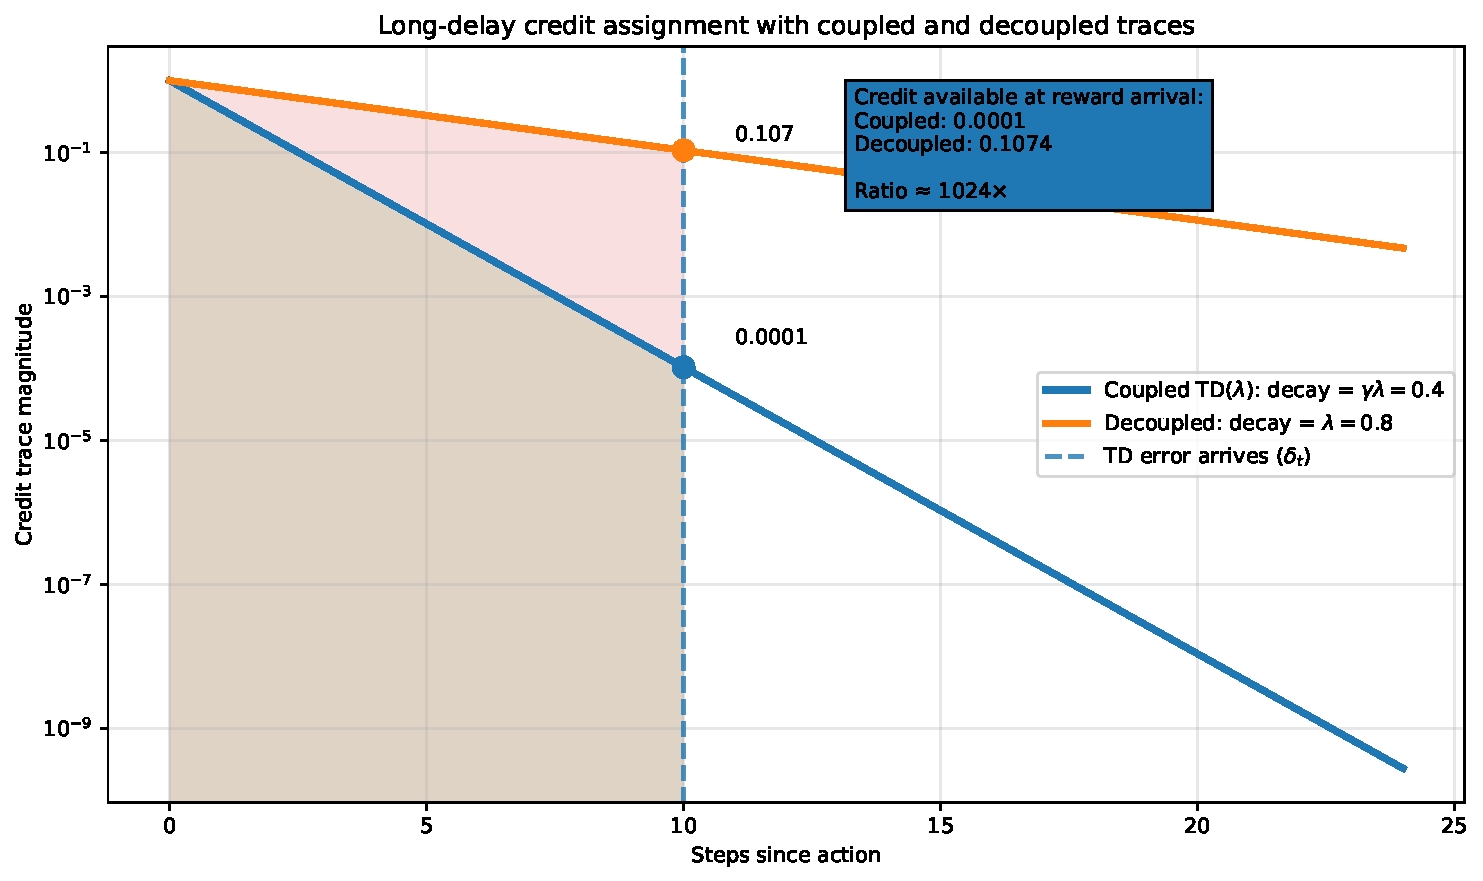
\includegraphics[width=0.45\linewidth]{images/credit_trace_comparison.pdf}
    \caption[Coupled vs.\ decoupled $\gamma
    ;\lambda$ credit traces]{Effect of coupling and decoupling $\gamma$ and $\lambda$ on temporal credit assignment. The figure shows the evolution of a credit trace following a single contribution at $t=0$. In the standard $TD(\lambda)$ formulation, the trace decays with factor $\gamma\lambda$, whereas in the proposed formulation it decays with factor $\lambda$ alone. For $\gamma=0.5$ and $\lambda=0.8$, the coupled trace rapidly approaches zero, leaving little credit available when a delayed TD error is observed. Decoupling the trace from the critic discount factor preserves a longer credit-assignment horizon while retaining the shorter value-estimation horizon required for stable learning.
    }
    \label{fig:gamma-lambda-decoupling-visualization}
\end{figure}

\subsection{Implementation in Multi-Step Action Windows}
\label{sec:multi-step-action}

The preceding discussion treats $\gamma$ and $\lambda$ as quantities defined at
the behavioral level, i.e. per agent action. In the simulations used in this
work, however, each action is maintained for $\Delta$ neural integration
steps. The corresponding per-step decay constants are therefore obtained by

\begin{equation}
\gamma_{\mathrm{step}} = \gamma^{1/\Delta},
\qquad
\lambda_{\mathrm{step}} = \lambda^{1/\Delta},
\end{equation}
so that the effective discount and credit-assignment horizons remain unchanged
when measured in units of actions.

Throughout the experiments we use $\gamma = 0.5$ and $\lambda = 0.8$ at the
action level. This choice reflects the role separation introduced above. A
relatively small $\gamma$ helps stabilize value learning in the continuous,
non-episodic spiking setting by limiting the critic's bootstrap horizon,
whereas a larger $\lambda$ preserves a substantially longer action-credit
window. Under the conventional coupling, the effective actor trace would decay
with $\gamma\lambda = 0.4$, producing a much shorter memory of past
action-related contributions. By decoupling the two constants, the critic can
remain short-horizon and stable while the actor continues to assign credit
across longer delays between actions and their consequences.

This modification should be viewed as a pragmatic design choice for online
spiking reinforcement learning, and shouldn't be seen as an exact implementation of
standard TD($\lambda$). Its motivation is to preserve useful long-range credit
assignment in regimes where critic stability requires strong discounting, and
its validity is ultimately assessed through the empirical results presented in
later chapters.


% ─────────────────────────────────────────────────────────────

\section{Distributed E-prop}
\label{sec:distributed_eprop}

The second contribution of this work is distributed e-prop, a learning rule that eliminates the need for structured feedback weights. Each neuron evaluates
its own contribution to the global outcome using only the broadcasted TD error $\delta_t$,
with no neuron-specific gradient routing.

   \subsection{Introduction: A Distributed View of Policy Optimization}
    \label{sec:distributed_eprop_intuition}
    
    Before presenting the formal derivation, it is helpful to situate distributed e-prop
    within a broader landscape of optimization strategies, and in particular to contrast it
    with the family of methods that backpropagation and standard e-prop belong to. This
    contrast motivates both the name and the design choices that follow.
    
    Backpropagation and its online approximations, including standard e-prop, share a common
    requirement: in order to update a parameter, the algorithm must know how that parameter
    influences the policy, that is, how the probability distribution over actions would
    change if that parameter were modified. In the policy gradient framework, this is
    captured by the score function $\nabla_\theta \log \pi(a \mid s; \theta)$, which
    measures the sensitivity of the log-probability of the selected action to each parameter.
    In backpropagation this quantity is computed by propagating gradients backward through
    the full network graph. In standard e-prop it is approximated by routing a
    neuron-specific signal back to each hidden neuron through feedback weights $B_{kj}^\pi$,
    so that each synapse receives an estimate of how its activity contributes to changing
    what the agent does. Note that the task signal, in the form of the temporal-difference
    error $\delta_t$, is present in both standard e-prop and distributed e-prop, it is not what distinguishes the two approaches. What distinguishes them is whether each parameter
    also receives structural information about how it influences the policy. It is precisely
    this structural signal, the approximation of $\nabla_\theta \log \pi$ routed back
    through the network, that distributed e-prop eliminates.
    
    A fundamentally different philosophy exists, one that abandons this structural accounting
    entirely and replaces it with a much simpler question: \emph{Was the outcome better or worse than expected, and what did I try?} This is the intuition behind evolutionary and
    perturbation-based optimisation methods such as genetic algorithms and evolution
    strategies~\cite{salimans2017evolutionstrategiesscalablealternative}. In these methods, candidate solutions are
    perturbed randomly, the resulting outcomes are evaluated, and perturbations that led to
    improvements are reinforced. No parameter needs to know how it influences the output
    through the network; it only needs to remember what perturbation it applied and whether
    the global outcome improved. The update rule is simply the product of the scalar outcome
    signal, shared identically across all parameters, and the local perturbation, which each
    parameter already knows because it generated it. The structural question of how each
    parameter shapes the policy is never asked; it is replaced by the empirical question of
    whether trying something different locally happened to coincide with a better outcome.
    
    Distributed e-prop is built on this same philosophy, adapted to work online and in
    continuous time within a recurrent spiking network. The key conceptual step is to treat
    each neuron not merely as a processing unit within a single global policy, but as an
    independent stochastic actor with its own local policy over its membrane dynamics.
    Concretely, each neuron $j$ maintains a Gaussian policy over its own membrane potential $v_j^t$, drawing a small
    random perturbation at each timestep and treating it's perturbed membrane as its local action.
    The spike train that results from those perturbed membrane dynamics constitutes the
    observable behavior that the perturbation produces, and it is through this behavior
    that the neuron influences the global outcome. In this sense the global agent policy
    emerges from the collective behavior of many small independent actors, each exploring
    locally, rather than from a single centralized computation whose gradient is then routed
    back to every parameter.
    
    Because the neurons integrate their inputs over time, a perturbation applied at time $t$ does
    not simply affect the membrane instantaneously and then vanish, its residual influence decays
    through the membrane dynamics over subsequent timesteps. Each neuron therefore maintains
    a filtered trace $\xi_j^t$ that accumulates the effect of its past perturbations on its
    current membrane state, decaying at the same rate $\alpha$ as the membrane itself. This
    trace serves as the neuron's local memory of what it has been trying recently, playing
    the same role that the stored perturbation plays in the static ES setting, but extended
    across time. When the global temporal-difference error $\delta_t$ arrives, each neuron
    uses its own $\xi_j^t$ to assess whether what it was trying recently contributed to the
    outcome being better or worse than expected, and updates its incoming weights accordingly.
    Crucially, \emph{no approximation of $\nabla_\theta \log \pi$ is needed at any point}, the
    structural question of how each neuron shapes the policy is replaced entirely by the
    empirical evidence accumulated in $\xi_j^t$.

    A natural question at this point is why this approach should work at all. If every
    parameter is being perturbed simultaneously, the change in the global outcome reflects
    the combined effect of thousands of simultaneous perturbations with residual influence over time, so attributing any part
    of that change to a single synapse seems hopeless. This concern is well founded, weight perturbation methods are known to suffer from variance that grows
    linearly with the number of parameters, precisely because every other perturbation
    contributes noise to the gradient estimate of each individual weight. The reason
    distributed e-prop can nevertheless be expected to produce a useful learning signal lies
    in two complementary mechanisms.
    
    The first is statistical. Even when all parameters are perturbed simultaneously, the
    expected value of the update for any single synapse $W_{ji}$ is still the correct
    gradient, because the perturbations of all other synapses are independent and
    zero-mean, and their contributions therefore cancel in expectation. What remains after
    averaging over many updates is the true gradient signal, sitting on top of noise whose
    magnitude is large but whose mean is zero. In this sense the law of large numbers is
    doing the essential work, no single update is reliable, but the correct direction
    accumulates steadily over time while the noise averages away.
    
   The second mechanism is structural, and it is what makes distributed e-prop
    qualitatively different from naive simultaneous perturbation. The core perturbation
    estimator already contains a natural credit assignment structure through the presynaptic
    activity, which conditions each synaptic update on whether neuron $i$ was recently
    active and therefore in a position to have contributed to the membrane state that the
    perturbation acted on. The single heuristic addition on top of this is the surrogate
    derivative $\psi_j^t$, which focuses credit further by weighting updates according to
    how close the postsynaptic neuron was to its firing threshold at each moment. The
    intuition is that a perturbation that occurs when the membrane is far from
    threshold is unlikely to have changed the spike output, and therefore unlikely to have
    influenced the global outcome, so it should receive little credit. Multiplying by
    $\psi_j^t$ implements exactly this reweighting, and the product of $\psi_j^t$ with the
    presynaptic activity is precisely the eligibility trace $e_{ji}^t$. This single
    heuristic introduction dramatically reduces the effective variance of the estimator at
    the cost of bias, and it is what makes the rule stable enough to operate online in
    a single continuous trajectory without requiring the large parallel populations that
    unbiased perturbation methods need.
    
    No neuron requires a centrally computed policy gradient, and no structured information
    about how the global policy depends on each parameter needs to be routed back through
    the network. The local signals that each neuron constructs can still propagate to other
    neurons, as in the backpropagated variants described in
    Section~\ref{subsec:structured_routing}, but their origin is always local and perturbation-based. The policy is in this
    sense distributed as it emerges from the independent stochastic behavior of many
    individual actors, each optimizing itself against the same shared scalar signal
    $\delta_t$.

    A final important observation concerns the role of the output weights. Throughout the
    recurrent and hidden layers, the weight updates are driven by noisy perturbation-based
    estimates that are only correct in expectation and over many steps. The output weights,
    by contrast, receive an exact gradient at every step, since the readout is a linear
    non-recurrent transformation and no approximation of the kind introduced by e-prop is
    needed there. The output weights are responsible for
    aggregating the activity of the hidden population into a value estimate and a policy
    signal, and it is the quality of this aggregation that determines how informative and
    stable the temporal-difference error $\delta_t$ is for the recurrent layer. Without the
    output weights learning a meaningful readout, $\delta_t$ would be extremely noisy,
    making it far harder for the perturbation correlations in the hidden layer to accumulate
    into a useful learning signal. Furthermore, if the output weights were fixed, the
    recurrent neurons would face a significantly harder problem, instead of the readout
    adapting to extract whatever structure the recurrent layer naturally develops, each
    hidden neuron would need to organize its activity to match an arbitrary fixed
    projection. Having the output weights learn the aggregation is therefore not merely
    convenient but arguably one of the most important factors in making the perturbation-based
    updates in the recurrent layer feasible. This is analogous to reservoir computing
    \citep{Maass2002LSM}, where a fixed random recurrent network can solve
    tasks because a trained linear readout learns to extract the relevant
    structure from the random recurrent dynamics.
    The key difference is that here the recurrent weights do learn, but the output weights
    play an arguably dominant role (particularly early in training), when the
    hidden representations are still unstructured. The recurrent learning can then be
    understood as a slow refinement of those representations, guided by a task signal whose
    quality depends heavily on how well the output layer has already learned to read them
    out.
    
    The sections that follow make this precise. Section~\ref{subsec:neuron_as_actor} formalises
    the interpretation of each neuron as a stochastic actor, and
    Section~\ref{subsec:lif_update_rule} describes the resulting update rule for LIF and ALIF
    neurons, showing how the perturbation trace $\xi_j^t$ and the e-prop eligibility trace
    $e_{ji}^t$ combine with $\delta_t$ to produce a fully local, online weight update.

    \subsection{Neurons As Stochastic Actors}
    \label{subsec:neuron_as_actor}
    
    As discussed previously, the non-local learning signal $L_j^t$ used in standard
    reward-based e-prop introduces an approximation to the true gradient, since
    estimating the contribution of each neuron to the global objective requires
    information about downstream network dynamics.
    One alternative is to reinterpret each neuron as an independent stochastic
    actor interacting with the rest of the recurrent network as its environment.
    Under this interpretation, learning can be performed using only local neuron
    dynamics, local stochastic exploration, and a globally broadcast evaluative
    signal.
    
    Instead of treating spikes themselves as stochastic actions, stochasticity is
    introduced directly into the membrane dynamics by treating the membrane
    potential as a stochastic actor.
    The emitted spikes remain deterministic threshold events.
    For each neuron $j$, the membrane potential is drawn from a Gaussian policy
    \[
        v_j^t \sim \mathcal{N}(\mu_j^t,\, \sigma_j^2),
    \]
    where $\mu_j^t$ is the unperturbed membrane state determined by the
    deterministic dynamics, and $\sigma_j^2$ is a per-neuron exploration variance.
    We write $\varepsilon_j^t = v_j^t - \mu_j^t$ for the additive perturbation,
    so that $\varepsilon_j^t \sim \mathcal{N}(0, \sigma_j^2)$.
    Under this formulation, the stochastic policy is defined over membrane
    trajectories.
    The perturbations therefore play the role of exploratory actions, while the
    resulting spike trains constitute the observable behavior generated by those
    actions.
    
    A key distinction from standard policy-gradient formulations is that the
    membrane potential itself is not directly observable by downstream neurons or
    by the environment.
    The observable quantity is instead the emitted spike train
    \[
        z_j^t = H(v_j^t - v_{\mathrm{th}}),
    \]
    where $H$ denotes the Heaviside Step function.
    Consequently, membrane perturbations only influence behavior insofar as they
    modify spike timing.
    
    \subsection{The Update Rule for LIF Neurons}
    \label{subsec:lif_update_rule}
    
    We first consider a network of leaky integrate-and-fire (LIF) neurons.
    The perturbed membrane dynamics are
    \[
        v_j^{t+1} = \alpha v_j^t + \sum_i W_{ji}\, z_i^t - z_j^t\, v_{\mathrm{th}}
                    + \varepsilon_j^t,
    \]
    where $\alpha$ is the membrane decay constant.
    The perturbation $\varepsilon_j^t$ enters additively into the membrane at each
    step, and its residual influence on the membrane at subsequent times decays at
    the same rate $\alpha$ as the membrane itself.
    We capture this accumulated influence by the filtered perturbation trace
    \[
        \xi_j^t = \alpha\, \xi_j^{t-1} + \varepsilon_j^t,
    \]
    so that $\xi_j^t$ represents the total contribution of all past perturbations
    to the current membrane state.
    
    The weight update is derived by correlating the local perturbation with the
    global return signal, following the evolution strategies approach.
    The score function of the Gaussian policy with respect to the mean $\mu_j^t$
    is $\varepsilon_j^t / \sigma_j^2$, which after temporal filtering gives
    $\xi_j^t / \sigma_j^2$.
    Chaining through $\partial \mu_j^t / \partial W_{ji} = \epsilon_{ji}^{t,v}$,
    the presynaptic eligibility vector, yields the gradient estimate
    \[
        \nabla_{W_{ji}} J
        \approx
        \mathbb{E}\!\left[
            \delta_t \cdot
            \frac{(1 - \alpha^2)\,\xi_j^t}{\sigma_j^2} \cdot
            \epsilon_{ji}^{t,v}
        \right],
    \]
    where $(1-\alpha^2)$ normalises for the stationary variance of the filtered
    perturbation process and $\delta_t$ is the broadcast TD error.
    
    This estimator correlates membrane perturbations with reward regardless of
    whether those perturbations actually caused a spike.
    A natural refinement is to weight the update by the sensitivity of the spike
    output to the membrane state, focusing credit on perturbations that were near
    threshold and thus likely to have modified spike timing.
    We therefore introduce $\psi_j^t$, the surrogate derivative of $H$ at
    $v_j^t$, as a heuristic modulation of the update: it is large near threshold
    and suppresses updates when the neuron is far from firing.
    Incorporating this term and recognising that $\psi_j^t \cdot \epsilon_{ji}^{t,v}$
    is precisely the e-prop eligibility trace $e_{ji}^t$ for LIF
    neurons~\cite{eprop2020}, the full update rule becomes
    \[
        \Delta W_{ji}
        \propto
        \delta_t\;
        \mathcal{F}_{\lambda}
        \!\left(
            \frac{(1 - \alpha^2)\, \xi_j^t}{\sigma_j^2}\;
            e_{ji}^t
        \right),
    \]
    where $\mathcal{F}_{\lambda}$ is a low-pass filter that accumulates credit
    over time.
    We note that the $\psi_j^t$ modulation is a choice,
    one could use the estimator without it, or apply other gating mechanisms (perhaps smoother functions), yielding
    valid alternative variants of the update rule, but, as it will be shown in Chapter~\ref{ch:results} this gating becomes essential for the rule to function properly.
    
    \paragraph{Extension to ALIF neurons.}
    For adaptive leaky integrate-and-fire (ALIF) neurons, the firing threshold
    depends on the neuron's recent spiking history through an adaptation variable
    $a_j^t$, giving the spike condition $z_j^t = H(u_j^t)$ where $u_j^t =
    v_j^t - A_j^t$ and $A_j^t = v_{\mathrm{th}} + \beta_j a_j^t$ is the adaptive
    threshold.
    The actor remains $v_j^t$, with the perturbation $\varepsilon_j^t$ injected
    into the membrane as before.
    The ES estimator is unchanged, still giving $\xi_j^t / \sigma_j^2 \cdot
    \epsilon_{ji}^{t,v}$ from the policy gradient.
    However, the e-prop framework also provides access to $\epsilon_{ji}^{t,a}$,
    the eligibility vector tracking the sensitivity of the adaptive threshold to
    $W_{ji}$ through the spiking history.
    Applying the same $\psi_j^t$ heuristic and extending it to include the
    adaptation contribution (which is natural since $\psi_j^t$ acts on $u_j^t =
    v_j^t - A_j^t$ and both membrane and adaptation dynamics feed into it) gives
    $\psi_j^t \cdot (\epsilon_{ji}^{t,v} + \epsilon_{ji}^{t,a})$, which is
    precisely the e-prop eligibility trace $e_{ji}^t$ for ALIF
    neurons~\cite{eprop2020}.
    The update rule therefore retains exactly the same form with $e_{ji}^t$
    reinterpreted accordingly.
    Including $\epsilon_{ji}^{t,a}$ is again a heuristic choice, one could omit
    it and use only $\epsilon_{ji}^{t,v}$, or include it with a different
    weighting, producing a family of possibly functional variants.
    
    \subsection{Intuitive Justification for the Eligibility Trace}
    \label{subsec:etrace_intuition}
    
    The update rule derived above combines three factors, $\delta_t$,
    $\xi_j^t / \sigma_j^2$, and $e_{ji}^t$, each playing a distinct and
    complementary role in local credit assignment.
    This section unpacks that decomposition to provide an intuitive justification
    for the use of the eligibility trace, independent of the heuristic argument
    that led to it.
    
    The TD error $\delta_t$ is a scalar signal broadcast uniformly to all neurons.
    It evaluates whether the global outcome was better or worse than expected under
    the current policy, and provides the evaluative signal that determines the sign
    and magnitude of all weight updates.
    It carries no information about which neurons or synapses were responsible for
    that outcome.
    
    The perturbation trace $\xi_j^t$ fills a different role entirely.
    It accumulates the causal footprint of past exploration noise on the current
    membrane state of neuron $j$, specifically how much the perturbations have
    cumulatively shifted the membrane away from what the deterministic dynamics
    alone would have produced, and in which direction.
    A large positive $\xi_j^t$ means the membrane has been pushed upward by
    recent noise; a large negative value means it has been pushed downward.
    Crucially, $\xi_j^t$ carries no evaluative content and does not encode whether
    those shifts were beneficial.
    That judgment is left entirely to $\delta_t$.
    Together, $\delta_t \cdot \xi_j^t / \sigma_j^2$ answers the question of whether
    the perturbations that drove this neuron's membrane in a given direction were
    followed by better or worse outcomes than expected.
    
    What remains is the question of which synapses should be updated in response.
    The perturbation entered through the membrane, and the membrane is a sum of
    contributions from all incoming synapses, so the perturbation's effect on the
    spike output was mediated by the same membrane dynamics that all synapses share.
    The eligibility trace $e_{ji}^t = \psi_j^t \cdot \epsilon_{ji}^{t,v}$ (or
    its ALIF counterpart $\psi_j^t \cdot (\epsilon_{ji}^{t,v} +
    \epsilon_{ji}^{t,a})$) provides the answer.
    It measures the sensitivity of the neuron's recent spike output to the
    synaptic weight $W_{ji}$, accumulated over time through the membrane dynamics,
    asking how much the spike activity of neuron $j$ would have differed if
    $W_{ji}$ had been slightly different.
    A synapse with large $|e_{ji}^t|$ was highly influential in shaping the
    membrane state that determined whether the perturbation produced a spike, while
    a synapse with small $|e_{ji}^t|$ had little influence, perhaps because the
    presynaptic neuron was silent or the membrane was far from threshold.
    
    The full update $\delta_t \cdot \xi_j^t / \sigma_j^2 \cdot e_{ji}^t$
    therefore has a clean three-factor interpretation. A synapse is strengthened
    or weakened when the global outcome was better or worse than expected
    ($\delta_t$), the membrane was being driven by exploration noise in a
    particular direction ($\xi_j^t$), and that synapse was causally responsible
    for the membrane state being sensitive to the spike output at that moment
    ($e_{ji}^t$).
   
    This structure is similar to the three-factor rules proposed in biological
    models of reward-modulated synaptic plasticity
    \citep{Fremaux2016NeuromodulatedSTDP}, where a neuromodulatory signal
    gates a Hebbian-like trace formed from correlated pre- and postsynaptic
    activity. The eligibility trace $e^t_{ji}$ inherited from standard e-prop
    plays exactly this role, and concrete biological instances of a global
    signal gating such as traces predate e-prop by over a decade
    \citep{Izhikevich2007DistalReward,Florian2007RewardSTDP}. The perturbation
    trace $\xi^t_j$ has no comparable precedent in this literature, since
    classical reward-modulated STDP rules do not model exploration as
    injected continuous noise; the closer biological precedent for this
    component is the conductance-fluctuation models of \citep{fiete2006gradient}, in which a REINFORCE-like estimator emerges directly
    from injected noise.
    
    \subsection{Synaptic Perturbation Variants}
    \label{subsec:synaptic_perturbation}
    
    The formulation above treats each neuron as a stochastic actor, injecting a shared
    membrane perturbation $\varepsilon_j^t$ that affects all incoming synapses
    simultaneously. This neuron perturbation variant has a natural bias-variance
    interpretation, that is because a single noise source is shared across all incoming synapses of
    neuron $j$, the gradient estimate for each individual synapse $W_{ji}$ is contaminated
    by the contributions of all other synapses to the membrane, since all of them
    experienced the same perturbation. The estimator cannot distinguish which synapse was
    responsible for the membrane shift; it only knows that the neuron as a whole was
    perturbed. This introduces bias into the per-synapse credit assignment, but keeps the
    number of independent noise sources equal to the number of neurons, which limits
    variance.
    
    A natural alternative is to push the stochasticity one level lower and treat each
    synapse as an independent actor. Rather than perturbing the membrane directly, a
    separate noise term $\varepsilon_{ji}^t \sim \mathcal{N}(0, \sigma_{ji}^2)$ is added
    to the synaptic transmission, so that the membrane dynamics become
    \[
        v_j^{t+1}
        =
        \alpha v_j^t
        +
        \sum_i \bigl(W_{ji} + \varepsilon_{ji}^t\bigr) z_i^t
        -
        z_j^t v_{\mathrm{th}}.
    \]
    The effective membrane perturbation produced by synapse $ji$ at time $t$ is therefore
    $\varepsilon_{ji}^t z_i^t$: the noise is only injected into the membrane when the
    presynaptic neuron fires. We define a per-synapse perturbation trace
    \[
        \xi_{ji}^t = \alpha\, \xi_{ji}^{t-1} + \varepsilon_{ji}^t z_i^t,
    \]
    which accumulates the residual influence of past synaptic perturbations on the current
    membrane potential, decaying at the same rate $\alpha$ as the membrane itself.
    
    Correlating the synaptic perturbation with the global return, the policy gradient with
    respect to $W_{ji}$ yields
    \[
        \nabla_{W_{ji}} J
        \approx
        \mathbb{E}\!\left[
            \delta_t \cdot
            \frac{(1 - \alpha^2)\, \xi_{ji}^t}{\sigma_{ji}^2}
            \; e_{ji}^t
        \right],
    \]
    where the eligibility trace $e_{ji}^t$ is introduced by the same heuristic argument as
    in the neuron variant. The resulting update rule is
    \[
        \Delta W_{ji}
        \propto
        \delta_t\;
        \mathcal{F}_{\lambda}
        \!\left(
            \frac{(1 - \alpha^2)\, \xi_{ji}^t}{\sigma_{ji}^2}\;
            e_{ji}^t
        \right).
    \]
    This variant resolves the bias of the neuron perturbation estimator: each synapse now
    has its own independent noise source and its own perturbation trace, so the gradient
    estimate for $W_{ji}$ depends only on the perturbation that synapse $ji$ itself
    introduced. However, this comes at the cost of a substantial increase in variance.
    The number of independent noise sources now scales with the number of synapses, which is typically one to two orders of magnitude larger.
    Each synapse contributes its own noise to the shared membrane potential of its
    postsynaptic neuron, and this noise affects the gradient estimates of all other synapses
    onto the same neuron.
    
    \paragraph{Shared postsynaptic noise with per-synapse structure.}
    
    A third variant addresses this variance problem by combining the strengths of the two
    approaches above. Rather than drawing an independent noise sample per synapse, a single
    noise term $\varepsilon_j^t \sim \mathcal{N}(0, 1)$ is drawn per postsynaptic neuron
    $j$ at each timestep, shared across all synapses that project onto $j$ and fire at time
    $t$. However, each synapse $ji$ scales this shared noise by its own per-synapse standard
    deviation $\sigma_{ji}$, so that the effective perturbation contributed by synapse $ji$
    is
    \[
        \varepsilon_{ji}^t z_i^t = \sigma_{ji}\, \varepsilon_j^t\, z_i^t.
    \]
    The per-synapse perturbation trace is then
    \[
        \xi_{ji}^t = \alpha\, \xi_{ji}^{t-1} + \sigma_{ji}\, \varepsilon_j^t\, z_i^t,
    \]
    and the update rule retains the same per-synapse structure as the fully independent
    variant:
    \[
        \Delta W_{ji}
        \propto
        \delta_t\;
        \mathcal{F}_{\lambda}
        \!\left(
            \frac{(1 - \alpha^2)\, \xi_{ji}^t}{\sigma_{ji}^2}\;
            e_{ji}^t
        \right)
    \]
    This variant can be understood as interpolating between the neuron and synaptic
    perturbation extremes. The noise originates at the postsynaptic neuron, as in the
    neuron perturbation variant, which limits the number of independent noise sources to
    the number of neurons and keeps variance under control. At the same time, each synapse
    retains its own $\sigma_{ji}$, so the effective perturbation magnitude is synapse-specific
    and the update structure remains fully per-synapse. The coupling of all synapses onto
    neuron $j$ through the shared $\varepsilon_j^t$ means that the noise simultaneously
    probes the contribution of all active presynaptic neurons at time $t$, testing whether
    their joint activity in the context of this particular postsynaptic neuron was
    beneficial, while the per-synapse $\sigma_{ji}$ and $z_i^t$ factors ensure that the
    resulting gradient estimate is still attributed individually to each synapse. This
    combination appears to offer the best empirical performance of the three variants, which
    we verify in the experimental results of Chapter~\ref{ch:results}.
    
    \subsection{Structured Routing of Local Policy Gradients}
    \label{subsec:structured_routing}
    
    The distributed rules derived so far use a purely global evaluative signal:
    all neurons receive the same broadcast TD error $\delta_t$, while credit
    assignment is performed locally through the perturbation traces and
    eligibility traces.
    This already defines a valid distributed perturbation-based learning rule.
    However, once each neuron is interpreted as a stochastic actor, the local
    perturbation estimator also defines a neuron-local policy-gradient signal.
    This makes it possible to reuse the structured credit-routing machinery of
    symmetric reward-based e-prop~\cite{eprop2020}.
    
    In standard reward-based e-prop, the learning signal routed back to neuron
    $j$ is formed by propagating output error gradients backward through the
    output weights.
    The perturbation-based formulation provides an analogous quantity: a local
    estimate of the policy gradient at each neuron, which can replace the
    externally computed output gradient in the symmetric e-prop routing mechanism.
    Here, since all synapses in the recurrent layer are treated symmetrically,
    the routing proceeds through the recurrent weights themselves, with no
    distinction between output and recurrent connections.
    
    For the neuron perturbation variant, the perturbation trace
    $\xi_j^t / \sigma_j^2$ defines the local stochastic policy-gradient estimator
    associated with neuron $j$.
    Applying the surrogate derivative $\psi_j^t$ yields the neuron-local policy
    signal
    \[
        g_j^t
        =
        \frac{(1-\alpha^2)\,\xi_j^t}{\sigma_j^2}\,
        \psi_j^t,
    \]
    which is then propagated backward through the recurrent weights, aggregating
    feedback from all postsynaptic neurons:
    \[
        L_j^t
        =
        \sum_{k}
        W_{kj}\,
        g_k^t.
    \]
    The resulting synaptic update takes the standard reward-based e-prop form
    \[
        \Delta W_{ji}
        \propto
        -\eta
        \sum_t
        \delta_t\,
        \mathcal{F}_{\lambda}
        \!\left(
            L_j^t\;
            e_{ji}^t
        \right),
    \]
    where the learning signal $L_j^t$ is shared across all incoming synapses of
    neuron $j$.
    
    In the synaptic perturbation variant, the local perturbation estimator exists
    at the level of each individual synapse, with $\xi_{ji}^t / \sigma_{ji}^2$
    serving as the per-synapse analogue of the neuron-level trace $\xi_j^t /
    \sigma_j^2$.
    Instead of aggregating these traces at the postsynaptic neuron before routing,
    the policy signal is formed directly at the synapse.
    This is consistent with the interpretation of $\varepsilon_{ji}^t z_i^t$ as a
    membrane perturbation for which synapse $ji$ is the sole culprit: just as the
    neuron perturbation $\varepsilon_j^t$ is a shared membrane push attributed to
    all incoming synapses jointly, the synaptic perturbation $\varepsilon_{ji}^t
    z_i^t$ is a membrane push attributed exclusively to a single synapse. Applying the surrogate derivative $\psi_j^t$ yields the synapse-local policy
    signal
    \[
        g_{ji}^t
        =
        \frac{(1-\alpha^2)\,\xi_{ji}^t}{\sigma_{ji}^2}\,
        \psi_j^t,
    \]
    which is then propagated backward through the recurrent weights, aggregating
    feedback from all postsynaptic neurons:
    \[
        L_{j}^t
        =
        \sum_{k}
        W_{kj}\,
        g_{kj}^t.
    \]
    The synaptic update therefore becomes
    \[
        \Delta W_{ji}
        \propto
        -\eta
        \sum_t
        \delta_t\,
        \mathcal{F}_{\lambda}
        \!\left(
            L_{j}^t\;
            e_{ji}^t
        \right).
    \]
    The key distinction from the neuron variant is that the policy signal $g_{ji}^t$
    is specific to each synapse through $\xi_{ji}^t$. The aggregation over postsynaptic neurons
    through the recurrent weights remains, as it does in the neuron variant.
    
    In both perturbation variants, the final update rule is identical in form to
    symmetric reward-based e-prop, a neuron-level or synapse-level learning signal
    is routed backward through the recurrent weights, multiplied by the eligibility
    trace $e_{ji}^t$, and modulated by the global TD error $\delta_t$.
    In standard e-prop, $L_j^t$ depends on externally supplied output gradients.
    Here, the learning signal is instead constructed internally from local
    perturbation-based policy-gradient estimates generated independently by each
    neuron or synapse.
    The framework therefore replaces explicit gradient feedback with distributed
    stochastic policy signals derived entirely from local dynamics and a globally
    broadcast evaluative signal.

    A natural extension of the structured routing variants described above is to incorporate
    an additional term into the noise reward trace that draws a more explicit analogy with
    backpropagation. Recall that the neuron-local policy signal $g_j^t$ and its backrouted
    aggregate $L_j^t = \sum_k W_{kj} g_k^t$ are already defined above. Incorporating $L_j^t$
    into the noise reward trace gives
    \begin{equation}
        p_{ji}^{\xi, t} = \lambda \, p_{ji}^{\xi, t-1}
        + e_{ji}^t \left(g_j^t + g_j^tL_j^t \right),
        \label{eq:rl_noise_trace_extended}
    \end{equation}
    
    where the additional term $e_{ji}^t g_j^t L_j^t$ modulates the update by
    the degree of agreement between the local policy signal of neuron $j$ and the
    backrouted aggregate of postsynaptic policy signals. When the two are aligned, the
    synapse receives a stronger update, since the local perturbation propagated its effect
    forward through the recurrent connections in a direction consistent with the
    perturbation activity of downstream neurons. When they disagree, the term attenuates
    the update. There is a clear connection with backpropagation and the chain rule, but, here it is used as a heuristic term, as it does not appear from the derivation. It can be seen as a variance reduction term, that focuses the updates on synchronized perturbations.
    
    \begin{figure}[H]
        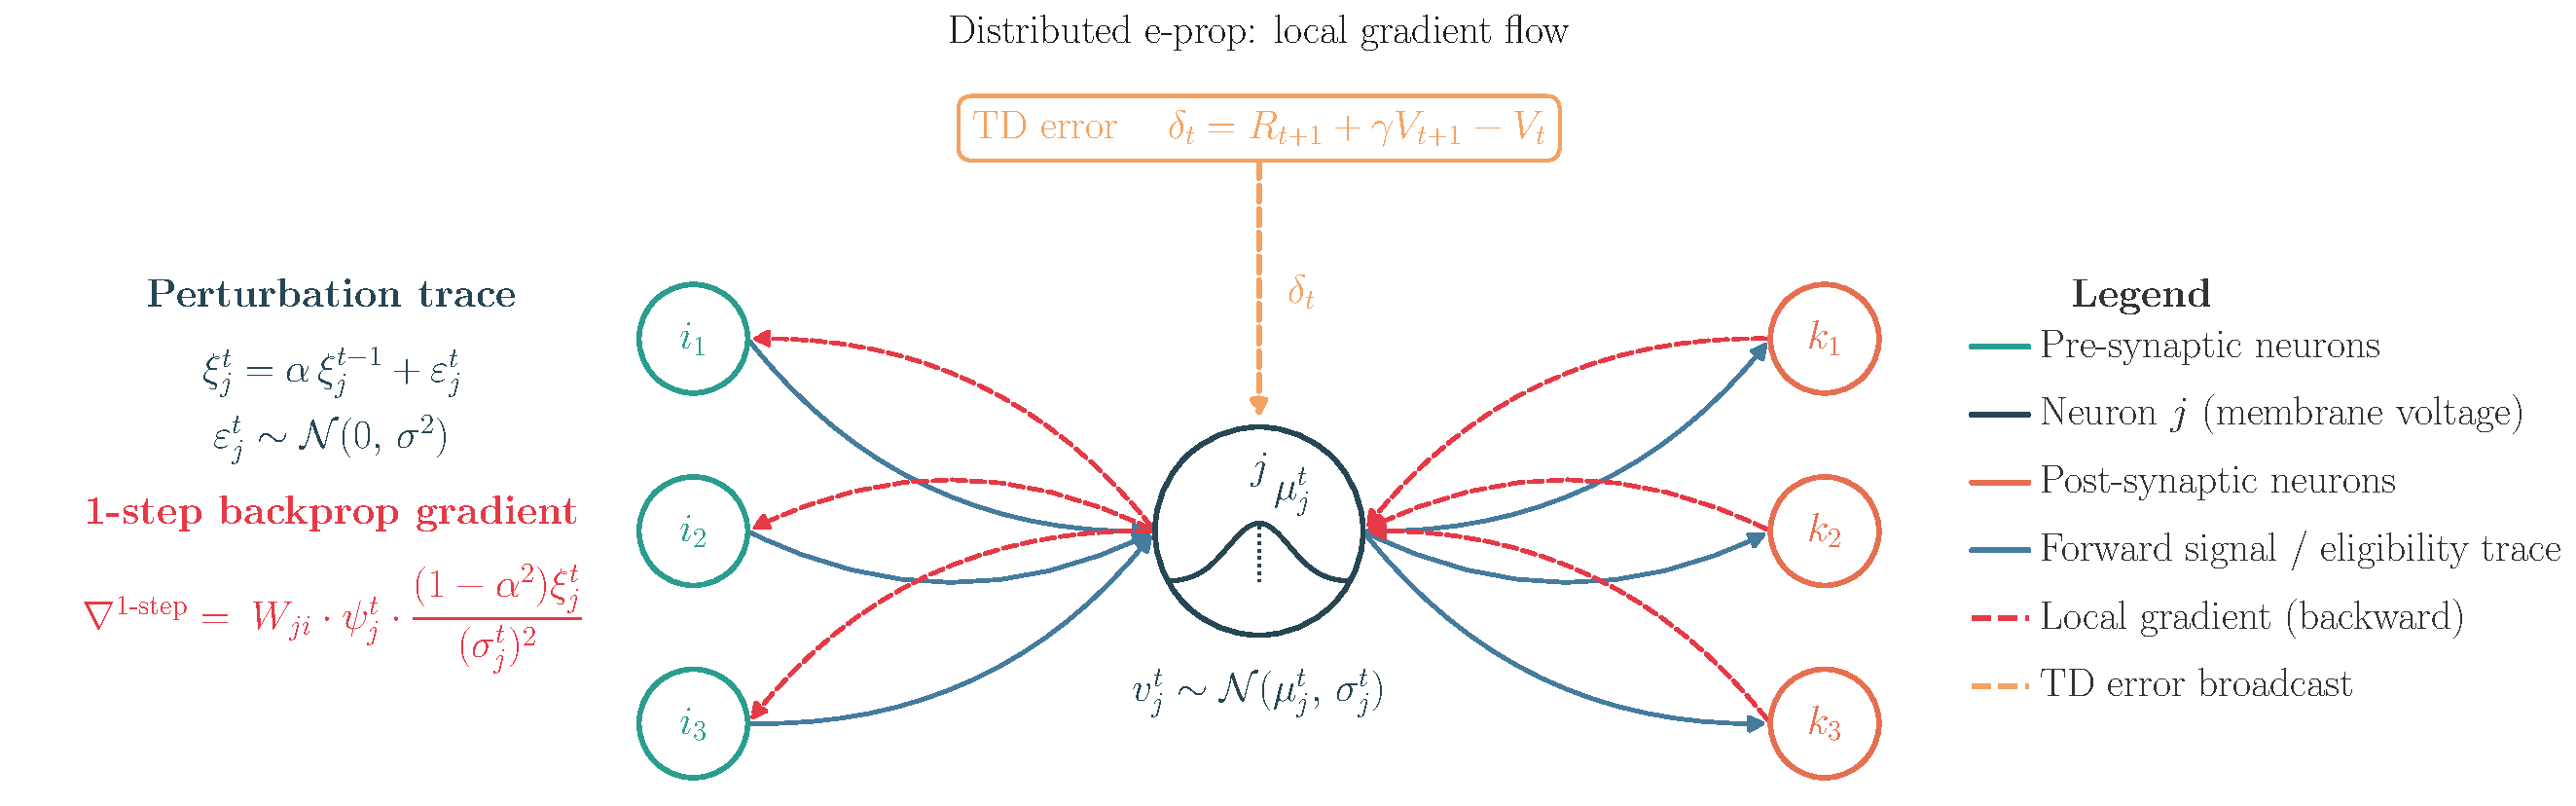
\includegraphics[width=1.0\linewidth]{images/distributed_eprop_diagram.pdf}
        \caption[Local gradient flow in distributed e-prop]{\textbf{Local gradient flow in the 1-step backpropagated distributed
        e-prop algorithm.}
        Neuron $j$ maintains an internal membrane voltage
        $v_j^t \sim \mathcal{N}(\mu_j^t, \sigma_j^t)$
        (represented by the Gaussian curve) and receives
        perturbation-based input from pre-synaptic neurons $i_1$--$i_3$
        (teal, left).
        The perturbation trace
        $\xi_j^t = \alpha\,\xi_j^{t-1} + \varepsilon_j^t$
        accumulates the stochastic exploration signal along each incoming
        synapse (blue arcs).
        Spikes $z_j^t$ are propagated forward to post-synaptic neurons
        $k_1$--$k_3$ (orange, right).
        A global TD error
        $\delta_t = R_{t+1} + \gamma V_{t+1} - V_t$
        is broadcast to the neuron from an external critic
        (orange dashed arrow).
        The 1-step backpropagation variant sends the local gradient information to their respective presynaptic neurons.
        }
        \label{fig:distributed_eprop}
    \end{figure}

    \clearpage
    \subsection{Exploration Variance \texorpdfstring{$\sigma$}{sigma}}
    \label{subsec:exploration_variance}
    
    The perturbation variance $\sigma_j^2$ controls the amount of local
    exploration performed by each neuron and plays a role analogous to the step
    size in stochastic search methods.
    Its choice has a direct effect on the bias-variance tradeoff of the gradient
    estimate: large $\sigma_j$ increases exploration but adds noise to the
    membrane dynamics and degrades network performance, while small $\sigma_j$
    reduces exploration and may prevent learning altogether.
    Three broad approaches can be taken.
    
    A static variance treats $\sigma_j$ as a fixed hyperparameter, either shared
    across all neurons or set individually.
    This avoids any additional learning machinery but requires manual tuning and
    cannot adapt as the policy evolves.
    In particular, a fixed $\sigma_j$ that is appropriate early in training, when
    the network is far from a good policy and wide exploration is beneficial, may
    be too large once a policy has been found and fine-grained exploitation is
    needed.
    A more expressive alternative makes $\sigma_j^t$ a function of the network
    state, for instance by reading it from a dedicated output neuron or by tying
    it to the membrane potential, allowing the network to modulate its own
    exploration in a context-dependent manner at the cost of a more complex
    architecture and additional credit assignment for the parameters governing
    $\sigma_j^t$.
    
    The third, and typically used approach, is to make $\log\sigma_j$ a
    per-neuron learnable scalar updated online by its own policy gradient.
    For the Gaussian policy $v_j^t \sim \mathcal{N}(\mu_j^t, \sigma_j^2)$,
    the score function with respect to $\log\sigma_j$ is
    \[
        \nabla_{\log\sigma_j} \log\pi_j
        =
        \frac{\varepsilon_j^{t\,2}}{\sigma_j^2} - 1,
    \]
    which has expectation zero under the current policy and is positive when the
    observed perturbation is larger than expected, indicating that increasing
    $\sigma_j$ would have been beneficial.
    Replacing the instantaneous perturbation with the filtered trace $\xi_j^t$
    and normalising for the stationary variance of the filtered process gives the
    online estimator
    \[
        s_j^t
        =
        \frac{(1-\alpha^2)\,(\xi_j^t)^2}{\sigma_j^2} - 1,
    \]
    which is accumulated over time and used to update $\log\sigma_j$ via
    \[
        \log\sigma_j
        \leftarrow
        \operatorname{clip}\!\left(
            \log\sigma_j + \eta_\sigma\, \delta_t\, s_j^t,\;
            \log\sigma_{\min},\;
            \log\sigma_{\max}
        \right),
    \]
    where $\eta_\sigma$ is a dedicated learning rate and the clipping enforces
    hard bounds on the exploration range.
    Parameterising in log space ensures $\sigma_j$ remains positive and makes the
    update scale-invariant with respect to the current value of $\sigma_j$.
    The update has an appealing interpretation: when $\delta_t > 0$ the outcome
    was better than expected, so the variance is increased if the perturbation was
    larger than typical (exploration was useful) and decreased otherwise; when
    $\delta_t < 0$ the signs reverse.
    In this way $\sigma_j$ adapts to the local curvature of the reward landscape
    as seen by each neuron independently.
    
    For the synaptic perturbation variant an analogous per-synapse update on
    $\log\sigma_{ji}$ can be defined using $\xi_{ji}^t$ in place of $\xi_j^t$.

    \subsection{Complete Update Rules with TD($\lambda$)}
    \label{subsec:complete_update_rules}
    
    We now consolidate the contributions of this section into a complete set of
    update rules, applying the TD($\lambda$) integration developed in
    Section~\ref{sec:decoupled-lambda-rule} to the distributed e-prop framework. The
    result is a family of fully online, local learning rules of increasing
    complexity, each building on the previous one by adding a new source of
    structured credit assignment. All rules are driven by the same globally
    broadcast TD error
    \begin{equation}
    \delta_t = R_{t+1} + \gamma V_{t+1} - V_t,
    \label{eq:complete-tderror}
    \end{equation}
    and differ only in the local trace that this error modulates.
    
    The value head is trained by standard TD learning. Its eligibility trace decays
    at rate $\gamma$ to remain consistent with the discounted bootstrap target,
    \begin{equation}
    \nu_{ji}^t = \gamma\, \nu_{ji}^{t-1} + \bar{z}_i^t,
    \qquad
    \Delta W_{ji}^V = \eta_V \sum_t \delta_t\, \nu_{ji}^t,
    \label{eq:complete-critic}
    \end{equation}
    where $\bar{z}_i^t$ is the filtered presynaptic spike train.
    
    The weights connecting the hidden population to the policy head are trained by a
    TD($\lambda$) rule whose credit trace accumulates the presynaptic activity
    weighted by the policy-gradient signal,
    \begin{equation}
    p_{ji}^{\pi,t} = \lambda\, p_{ji}^{\pi,t-1}
    + \bar{z}_i^t \, \nabla_{y_k^t} \log \pi^t(a_t),
    \qquad
    \Delta W_{ji}^\pi = \eta_\pi \sum_t \delta_t\, p_{ji}^{\pi,t},
    \label{eq:complete-policy}
    \end{equation}
    where $y_k^t$ are the output logits. The policy-gradient signal is directly
    available at the output head; the trace simply accumulates it over time
    weighted by $\lambda$, after which $\delta_t$ modulates it exactly as for every
    other weight in the network.
    
    The remaining (hidden and recurrent) weights all share a single update form,
    \begin{equation}
    \Delta W_{ji} = \eta \sum_t \delta_t\, p_{ji}^{\,t},
    \qquad
    p_{ji}^{\,t} = \lambda\, p_{ji}^{\,t-1} + c_{ji}^{\,t},
    \label{eq:master-update}
    \end{equation}
    and differ only in the instantaneous credit term $c_{ji}^{\,t}$. Two local
    signals enter these terms: the neuron-local policy signal
    \begin{equation}
    g_j^t = \psi_j^t\,(1-\alpha^2)\,\xi_j^t / \sigma_j^2,
    \label{eq:local-policy-signal}
    \end{equation}
    defined in Section~\ref{subsec:structured_routing}, and its backrouted
    aggregate
    \begin{equation}
    \Lambda_j^t = \sum_k W_{kj}\, g_k^t,
    \label{eq:backrouted-aggregate}
    \end{equation}
    which sums the local policy signals of all postsynaptic neurons weighted by the
    recurrent weights. The backrouted aggregate $\Lambda_j^t$ can enter the update
    in two distinct ways: \emph{additively}, as a separate routing trace, or
    \emph{multiplicatively}, gating the perturbation credit itself. The family of
    rules is obtained by the following choices of $c_{ji}^{\,t}$:
    
    \begin{table}[h]
    \centering
    \renewcommand{\arraystretch}{1.6}
    \begin{tabular}{@{}lll@{}}
    \toprule
    \textbf{Variant} & \textbf{Credit term $c_{ji}^{\,t}$} & \textbf{Decay} \\
    \midrule
    Local perturbation (base)
      & $e_{ji}^t\, g_j^t$
      & $\lambda_\xi$ \\
    \addlinespace
    + structured routing
      & $e_{ji}^t\, g_j^t$ \; and \; $e_{ji}^t\, \Lambda_j^t$ \;(separate trace)
      & $\lambda_\xi,\ \lambda_L$ \\
    \addlinespace
    + gating by structured routing
      & $e_{ji}^t\, g_j^t\,(1 + \Lambda_j^t)$ \; and \; $e_{ji}^t\, \Lambda_j^t$
      & $\lambda_\xi,\ \lambda_L$ \\
    \bottomrule
    \end{tabular}
    \caption{The family of hidden-weight update rules, expressed as choices of the
    instantaneous credit term $c_{ji}^{\,t}$ in Equation~\eqref{eq:master-update}.
    Each rule adds structure to the previous one.}
    \label{tab:update-variants}
    \end{table}
    
    The base rule, the most local one, makes it so each synapse relies entirely on its
    own perturbation trace and the shared scalar $\delta_t$, with no information
    flowing between neurons beyond the recurrent dynamics themselves. The
    structured-routing variant adds the backrouted signal $\Lambda_j^t$ as a second
    trace; because the perturbation trace and the routing trace play conceptually
    distinct roles and may benefit from different temporal horizons, their decays
    $\lambda_\xi$ and $\lambda_L$ may be set independently, with
    $\lambda_\xi = \lambda_L = \lambda$ recovering a single decay constant. The
    combined variant additionally lets $\Lambda_j^t$ \emph{gate} the perturbation
    credit through the factor $(1 + \Lambda_j^t)$, modulating it by the agreement
    between the local policy signal and the aggregate of postsynaptic signals.
    
    When two traces with different decays contribute, the per-synapse credit is
    their sum, $p_{ji}^{\,t} = p_{ji}^{\xi,t} + p_{ji}^{L,t}$, each evolving by
    Equation~\eqref{eq:master-update} with its own decay. For the shared
    postsynaptic-noise variant, $\xi_j^t$ is replaced by the per-synapse trace
    $\xi_{ji}^t = \alpha\,\xi_{ji}^{t-1} + \sigma_{ji}\,\varepsilon_j^t\,z_i^t$ and
    $\sigma_j^2$ by $\sigma_{ji}^2$ throughout.
    
    The exploration variance $\sigma_{ji}$ can itself be updated online by its own
    policy gradient (Section~\ref{subsec:exploration_variance}). The score function
    with respect to $\log \sigma_{ji}$ accumulates a credit trace analogous to those
    above,
    \begin{equation}
    s_{ji}^t = \lambda_\sigma\, s_{ji}^{t-1}
    + \frac{(1 - \alpha^2)\,(\xi_{ji}^t)^2}{\sigma_{ji}^2} - 1,
    \label{eq:sigma-trace}
    \end{equation}
    whose instantaneous term is the score function of the Gaussian policy with
    respect to $\log \sigma_{ji}$: it has expectation zero under the current policy
    and is positive when the observed perturbation was larger than expected. The
    update is
    \begin{equation}
    \log \sigma_{ji} \leftarrow \mathrm{clip}\!\left(
    \log \sigma_{ji} + \eta_\sigma\, \delta_t\, s_{ji}^t,\;
    \log \sigma_{\min},\; \log \sigma_{\max}
    \right),
    \label{eq:sigma-update}
    \end{equation}
    where $\eta_\sigma$ is a dedicated learning rate and the clipping enforces hard
    bounds on the exploration range. Parameterising in log space keeps
    $\sigma_{ji}$ positive and makes the update scale-invariant in its current
    value. The neuron-level rule of Section~\ref{subsec:exploration_variance}
    follows as the special case in which $\sigma_j$ is shared across all incoming
    synapses of neuron $j$, replacing $\xi_{ji}^t$ by $\xi_j^t$ accordingly.

    \subsection{Regularization}
    \label{subsec:regularization}
    
    Effective online learning in spiking networks requires mechanisms to prevent
    pathological activity patterns from developing over the course of training. Without
    any constraint on firing rates or membrane dynamics, neurons can drift toward sustained
    high-frequency spiking or toward silence, both of which degrade the quality of the
    eligibility traces and destabilize the learning signal. This section describes the
    regularization terms used in the distributed e-prop framework, which combine the
    standard e-prop firing rate regularization with reward-based variants for both firing
    rate and voltage that are native to the perturbation framework.
    
    \paragraph{Firing rate regularization.}
    
    The base firing rate regularization term is imported directly from standard e-prop
    \cite{eprop2020}. A filtered estimate of the average firing rate of each neuron,
    $F_j^{\mathrm{avg}}$, is maintained online and penalized for deviating from a target
    rate $F^*$. The regularization contribution to the weight update is
    \[
        \Delta W_{ji}^{\mathrm{reg}} = -\eta_{\mathrm{reg}}\,
        (F_j^{\mathrm{avg}} - F^*)\, e_{ji}^t,
    \]
    where $e_{ji}^t$ is the instantaneous eligibility trace. This term penalizes synapses
    whose postsynaptic neuron fires too frequently or too rarely relative to the target,
    pushing the network toward a regime where the eligibility traces remain informative and
    sparse spiking dynamics are preserved.
    
    In addition to this standard term, a reward-based firing rate regularization is
    introduced that exploits the perturbation framework. A slower trace
    $\bar{F}_j^{\mathrm{avg}}$ accumulates the absolute firing rate deviation over a
    longer timescale:
    \[
        \bar{F}_j^{\mathrm{avg},t} = \lambda\, \bar{F}_j^{\mathrm{avg},t-1}
        + (1 - \lambda)\, |F_j^{\mathrm{avg}} - F^*|.
    \]
    The difference between this slower trace and the current absolute deviation,
    \[
        r_j^{F,t} = \bar{F}_j^{\mathrm{avg},t} - |F_j^{\mathrm{avg}} - F^*|,
    \]
    measures whether recent activity has improved or worsened the firing rate regularity
    relative to a longer-horizon baseline. When $r_j^{F,t} > 0$, the recent firing
    pattern has brought the neuron closer to its target rate than the historical average,
    and the perturbations that contributed to this improvement are reinforced through the
    local perturbation traces. When $r_j^{F,t} < 0$, the recent activity has worsened
    regularity and the perturbation traces are suppressed. The corresponding weight update
    is
    \[
        \Delta W_{ji}^{F\text{-rew}} = -\eta_{\mathrm{reg}}\,
        r_j^{F,t}\, p_{ji}^{\xi,t},
    \]
    where $p_{ji}^{\xi,t}$ is the local perturbation credit trace defined in
    Section~\ref{subsec:complete_update_rules}. Note that only the local perturbation
    trace is used here, without the back-routed structured routing signal $p_{ji}^{L,t}$,
    since firing rate regularity is a property of the individual neuron and does not
    require information from downstream neurons to be corrected.
    
    \paragraph{Voltage regularization.}
    
    A voltage regularization term penalizes membrane potentials that deviate excessively
    from the firing threshold in either direction. The voltage deviation is defined as
    \[
        V_j^{\mathrm{reg},t} =
        \max(0,\, v_j^t - A_j^t)
        + \max(0,\, -v_j^t - A_j^t),
    \]
    where $A_j^t = v_{\mathrm{th}} + \beta a_j^t$ is the adaptive threshold. This quantity
    is positive whenever the membrane is far from threshold in either direction. Voltage
    is a continuous membrane quantity that does not manifest directly in spike space, and
    the eligibility trace, being driven by $\psi_j^t$ and the presynaptic spike filter, is
    naturally insensitive to voltage deviations that never produce a spike. The perturbation
    trace, by contrast, lives in membrane space and accumulates the residual influence of
    past perturbations on the current membrane state, making it the natural vehicle for
    voltage regularization. The corresponding weight update is therefore
    \[
        \Delta W_{ji}^{V\text{-reg}} = -\eta_V\,
        V_j^{\mathrm{reg},t}\, p_{ji}^{\xi,t},
    \]
    again using only the local perturbation trace, since
    voltage regularization is a local membrane phenomenon that terminates at the neuron.
    
    This is in contrast to a voltage regularization applied in the style of standard
    e-prop, which would take the form
    \[
        \Delta W_{ji}^{V\text{reg}} = -\eta_V\,
        V_j^{\mathrm{reg},t}\,
        \left( \bar{z}_i^t - \beta \epsilon_{ji}^{a,t} \right),
    \]
    operating directly on the voltage-space eligibility components. We attempted this
    formulation but found empirically that it caused membrane voltages to explode. The likely cause is that when the membrane is chronically far from
    threshold, $\psi_j^t$ is small and the perturbation traces carry little signal,
    naturally suppressing the update in exactly the pathological regime. The standard
    e-prop style term lacks this gating mechanism and can therefore generate large and
    poorly directed weight updates in regimes where the gradient estimate is unreliable,
    producing runaway positive feedback dynamics.
    
    \paragraph{Propagation of local regularization signals.}
    
    All regularization terms described above are strictly local, they depend only on the
    activity of the postsynaptic neuron and do not use any back-routed information from
    downstream neurons. This is a deliberate choice, since firing rate and voltage
    regularity are properties of individual neurons that can be assessed and corrected
    without reference to the global network state. However, within the distributed e-prop
    framework it is natural to ask whether these local regularization rewards could
    themselves be propagated to other neurons through the structured routing machinery of
    Section~\ref{subsec:structured_routing}, allowing neurons to coordinate their regularization
    behavior in a distributed manner. Preliminary experiments with this extension have
    shown promising results, but a systematic investigation is beyond the scope of this
    work and is left for future study.
    
\section{Network Architecture}
\label{sec:network-architecture}

\subsection{Excitatory-Inhibitory Recurrent Core}
\label{sec:ei_core}

The agent's hidden core is a recurrent spiking network organized according to an
excitatory-inhibitory (EI) scheme inspired by the observed structure of cortical
circuits. In biological neural tissue, neurons respect Dale's principle
\cite{dale1935pharmacology}: each neuron releases the same set of neurotransmitters
at all of its synapses, so that a given neuron acts either exclusively as an excitatory
or exclusively as an inhibitory unit across all of its postsynaptic targets. This
constraint gives rise to a structural separation between two functionally distinct
populations. The balance between these two populations yields an excitatory-inhibitory balance that has been shown to be a key
factor in stabilizing network dynamics, regulating firing rates, and enabling the
propagation of structured activity patterns over time \cite{vanVreeswijk1996Chaos}.

Following this organization, the hidden units are split into a separate excitatory (E)
population and an inhibitory (I) population, each laid out on its own two-dimensional
sheet. In our configuration this corresponds to a $20 \times 20$ excitatory grid and a
$15 \times 15$ inhibitory grid, each replicated over the input channels. The sign of
every connection is fixed by the type of its presynaptic population: excitatory neurons
project with positive weights and inhibitory neurons with negative weights, so that
Dale's principle holds at initialization. Within a layer, all four type-conditioned
connections are instantiated: $E \to E$ and $E \to I$ with positive sign, and $I \to E$
and $I \to I$ with negative sign.

Both populations are modelled as adaptive leaky integrate-and-fire (ALIF) neurons. In
addition to the membrane potential with time constant $\tau_m$, each neuron carries a
slow adaptive threshold variable with time constant $\tau_\text{adapt} \gg \tau_m$ and
adaptation strength $\beta$. This slow adaptation furnishes the network with long
intrinsic time constants that e-prop's eligibility traces can exploit for temporal
credit assignment. The neuron parameters are shared
across the two populations and summarised in Table~\ref{tab:hyperparams}.

How strictly Dale's principle should be enforced during training, and the empirical
consequences of different choices, are discussed in Section~\ref{sec:weakened_dale}.

\subsection{Depth and Per-Head EI Layers}
\label{sec:depth_ei}

Although the smallest useful configuration is a single recurrent EI population, the
architecture is modular. The EI block can be replicated into a stack of $L$ layers,
with recurrent connectivity inside each layer and feedforward EI projections carrying
activity from one layer to the next. The same connectivity and sign rules apply within
and between layers, so the EI structure is preserved as depth grows and representational
capacity can be scaled without changing the qualitative organization of the network.

On top of the shared core, each output head can be preceded by its own dedicated field
layer. Rather than reading the policy and value outputs directly from the core, a
separate population is interposed between the core and each head: a policy field and a
value field. Two motivations drive this choice. First, the actor and critic objectives
can pull the shared core representation in conflicting directions, since a weight change
that improves the value estimate may degrade the policy and vice versa. Giving each
head a private layer provides a buffer that absorbs some of this interference, leaving
the core free to develop a more general representation of the task state. Second, the
per-head layers give the actor and critic the capacity to develop specialized
representations tailored to their respective objectives, instead of forcing both to
read from the same population with no intermediate processing.

Each field is a population of ALIF neurons with the same shape as the inhibitory
population of the core, and receives feedforward connections from the last recurrent
layer through the same toroidal Gaussian connectivity strategy described in
Section~\ref{sec:toroidal}. Unlike the core layers, the field has no
recurrent connections within itself, it acts as a non-recurrent feedforward stage that
transforms the core's output into a representation suited to its respective head. Each
field is then densely connected to its own head, and the heads themselves are linear,
non-spiking leaky-integrator readouts. The policy head emits $N_\text{out}$
outputs (one per discrete action, normalized by a softmax for action selection) and
the value head a single scalar. Because the readout weights are not type-constrained,
Dale's law is applied only up to the field populations, not to the final readout.

It should be noted that this design introduces depth into the spiking architecture,
and depth poses a known difficulty for eligibility-trace based learning algorithms.
The eligibility traces themselves remain locally correct at each synapse regardless
of depth. The challenge lies instead in the feedback pathways, in standard e-prop,
the learning signal $L^t_j$ must be routed back through an additional population,
which increases the bias introduced by the random feedback projection. In distributed
e-prop, the field layer adds an extra stage over which the perturbation correlations
between the scalar $\delta^t$ and the local traces must develop, making those
correlations noisier and harder to exploit. In practice the dedicated layers appear
to provide a modest stabilizing effect on the value function, but this architecture
should be understood as a deliberate choice to study settings where the algorithms may struggle, as these are the settings where new approaches should be explored.

\subsection{Causal Path Length}
\label{sec:causal-path-length}

Throughout this work we make frequent reference to the \emph{causal path
length} between two neurons, by which we mean the shortest path between them
in the directed graph defined by the network connectivity. In a single-layer
network this distance is one for any neuron directly connected to an output
head; it increases as depth grows, and can be forced to increase further by
introducing hidden layers that connect only recurrently within themselves and
not across layers, so that any signal must pass through multiple intermediate
neurons before reaching the output.

This quantity is particularly relevant when comparing learning rules that
differ in how they route credit back through the network. Rules that rely on
structured feedback projections accumulate approximation error with each
additional step in the path, since the feedback signal is an increasingly
coarse approximation of the true gradient the further it must travel from
the output. The most extreme case is symmetric e-prop, whose feedback weights
are tied directly to the forward output weights, so any neuron that is not
directly connected to an output head receives no feedback signal whatsoever,
meaning that symmetric e-prop is not merely degraded by increasing causal
path length but fails entirely as soon as the path length exceeds one.
Random and adaptive e-prop are more robust in this respect, since feedback reaches all neurons, but it still accumulates approximation error with depth. Rules that
bypass policy feedback entirely, such as distributed e-prop, avoid this source of
error, but face a different challenge, as causal path length increases, a
single neuronal activation propagates its influence through a growing number
of downstream neurons before reaching the output, meaning that the change in
reward caused by any one perturbation becomes an increasingly entangled
function of many simultaneous perturbations. The correlation between a
neuron's local perturbation trace and the global reward signal therefore
weakens with causal path length, making it progressively harder for the
learning rule to extract a reliable credit assignment signal from the
broadcast scalar alone.

Whether structured feedback or perturbation-based credit assignment is
preferable is therefore not a question with a known answer, it could well be 
a bias-variance tradeoff whose outcome depends on the specific task,
network depth, and training budget.

\subsection{Toroidal Gaussian Connectivity}
\label{sec:toroidal}

All structural (sign-constrained) connections are sparse and spatially
organized, following a similar design to prior spiking network models with
toroidal, distance-dependent connectivity \citep{Spreizer2019Toroidal}.
Each neuron occupies a position on its sheet, with coordinates normalized
to the unit square $[0, 1]^2$ and an optional channel index.
For a
postsynaptic neuron at $(x,y)$, presynaptic partners are drawn by sampling
spatial offsets from an isotropic Gaussian and wrapping them periodically,
%
\begin{equation}
(\Delta x, \Delta y) \sim \mathcal{N}\!\left(0, \sigma^2 I\right),
\qquad
(x', y') = \big( (x + \Delta x)\bmod 1,\; (y + \Delta y)\bmod 1 \big),
\label{eq:toroidal-sampling}
\end{equation}
%
mapping each sampled location to its nearest grid neuron and removing
duplicates and self-connections. The modulo operation imposes
periodic (toroidal) boundary conditions, the sheet wraps in both
dimensions, so neurons near an edge connect across to the opposite edge. This
eliminates the boundary artefacts of a bounded sheet (under-connected edges
and corners) and renders the connection statistics approximately
translation-invariant.

The width $\sigma$ sets the spatial reach, small $\sigma$ yields locally
clustered, topographic connectivity and large $\sigma$ approaches uniform
random connectivity. We use a broader profile for the input projection
($\sigma_{\text{in}} = 0.1$) than for the recurrent connections
($\sigma_{\text{h}} = 0.05$), so that sensory input is distributed more widely
while recurrent processing remains local. Each postsynaptic neuron receives a
target fan-in of $K$ afferents (on the order of $K \approx 100$ in our
experiments). The fan-in may additionally be graded with distance from a
configurable centre $(c_x, c_y)$ via a power-law profile,
%
\begin{equation}
K(d) \;=\; \frac{K}{1 + (d/d_0)^{p}},
\qquad
d = \sqrt{(x - c_x)^2 + (y - c_y)^2},
\qquad p = 2,
\label{eq:fanin-decay}
\end{equation}
%
which we apply to the input projection (with scale $d_0 = 0.25$) to concentrate
afferents near the centre of the field; setting $d_0 \to \infty$ recovers a
spatially uniform fan-in $K$, as used for the recurrent connections.
\begin{figure}[h]
    \centering
    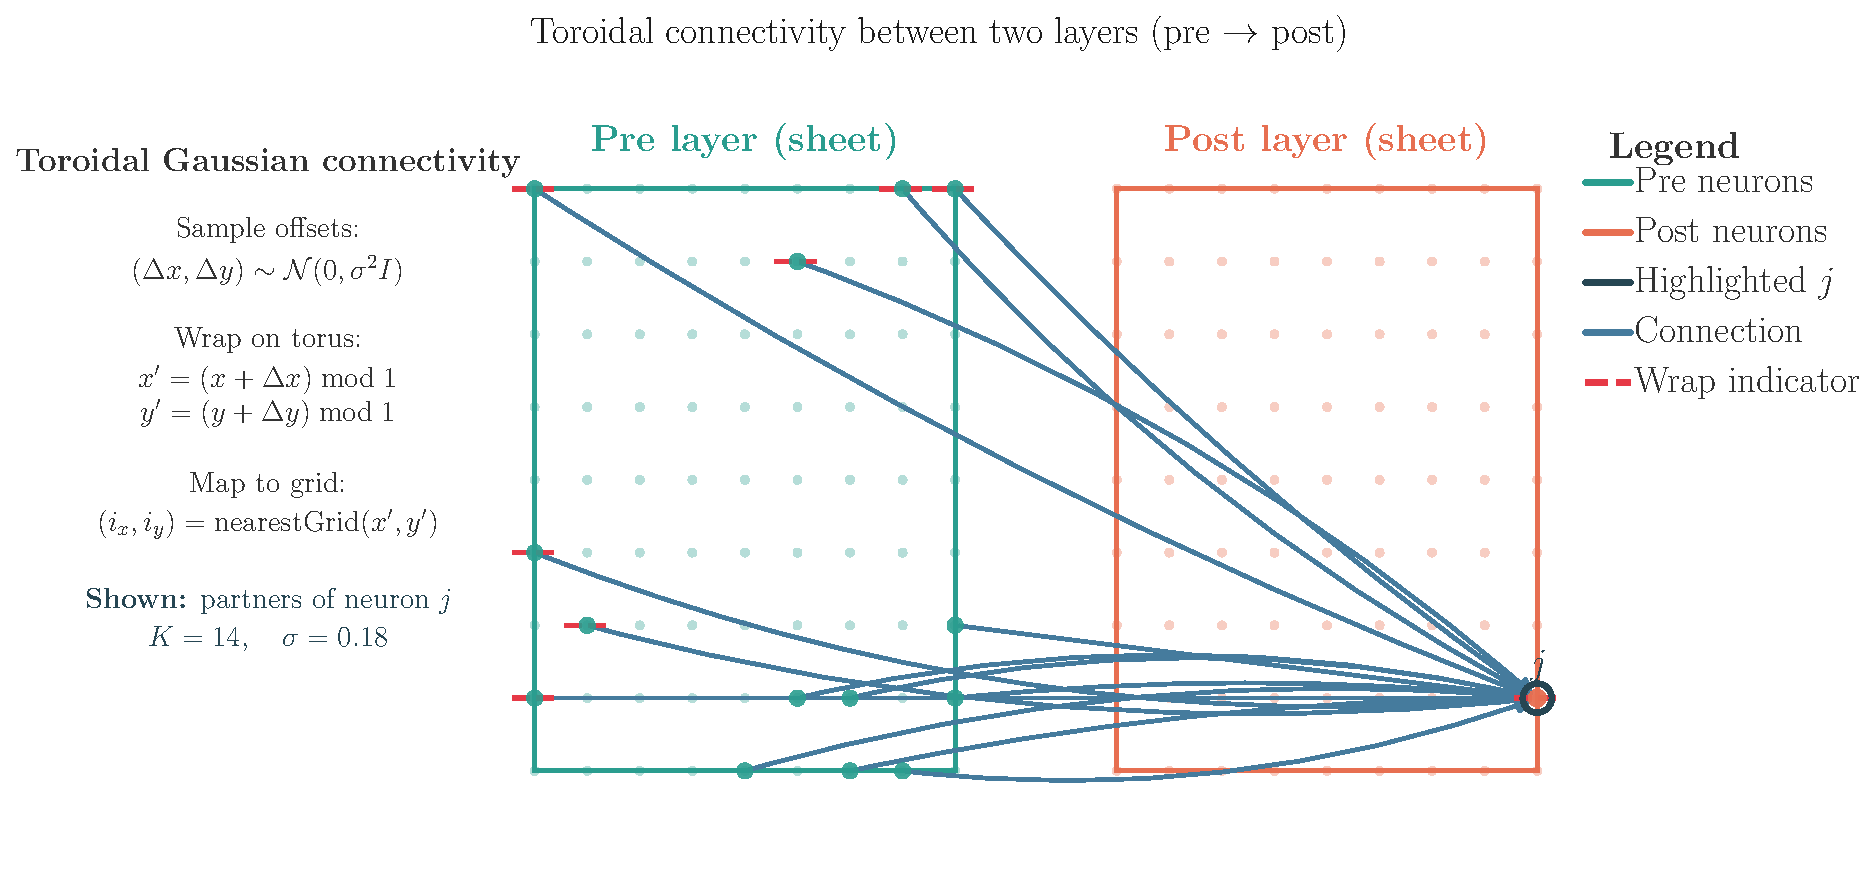
\includegraphics[width=1\linewidth]{images/toroidal_connectivity_two_layers.pdf}
    \caption[Toroidal Gaussian connectivity scheme]{
        \textbf{Toroidal Gaussian connectivity between the pre- and
        post-synaptic layers.}
        Each neuron $j$ in the post-synaptic layer (orange, right) receives
        input from $K$ pre-synaptic neurons (teal, left) sampled according
        to a 2-D Gaussian centred on the position of $j$ in the sheet.
        Offsets $(\Delta x, \Delta y)\sim\mathcal{N}(0,\sigma^2 I)$ are
        drawn in normalized coordinates $[0,1)^2$ and wrapped toroidally,
        so neurons near one border can connect to neurons near the opposite
        border; such wrap-around connections are indicated by dashed red
        markers.
        The sampled offset is then mapped to the nearest grid index,
        yielding a spatially structured but stochastic receptive field.
    }
    \label{fig:toroidal_connectivity}
\end{figure}

\clearpage
\subsection{Weight initialization}
\label{sec:weight-init}

Initial weights are drawn from a Gaussian whose mean and standard deviation
are scaled by the fan-in,
%
\begin{equation}
W_{ji} \sim \mathcal{N}\!\left( \mu, \, s^2 \right),
\qquad
\mu = \mathrm{sign}(i)\,\frac{c}{\sqrt{K}},
\qquad
s = \frac{\sigma_w}{\sqrt{K}},
\label{eq:weight_init}
\end{equation}
%
where $\mathrm{sign}(i) \in \{+1, -1\}$ is the Dale sign of the presynaptic
population. The $1/\sqrt{K}$ scaling makes the expected total synaptic drive
onto a neuron independent of its fan-in and of the layer width, keeping input
currents, and hence firing rates, in a stable operating range across
populations of different size and across depth, which prevents the saturation
or silencing that would otherwise impede the propagation of eligibility
traces. The mean magnitude $c$ is set asymmetrically for the two types:
excitatory connections use a small mean ($c_E = 0.1$), whereas inhibitory
connections use a substantially larger mean ($c_I = 3$). This asymmetry
restores the excitatory-inhibitory balance because the inhibitory population
is smaller, boosting the per-synapse inhibitory weight
ensures that the net inhibitory and excitatory drive onto a typical neuron are
comparable at initialization. The dispersion is common to both
($\sigma_w = 0.05$). Unconstrained readout and feedback connections, which
carry no Dale sign, are initialized with zero mean and a variance scaled by
the number of output units, $s = 1/\sqrt{N_{\text{out}}}$.

\subsection{A Weakened Dale's Law}
\label{sec:weakened_dale}

Dale's principle is imposed only at initialization. Every hidden neuron is assigned a
type, and through Equation~\ref{eq:weight_init} its outgoing weights take the
corresponding sign, so the network begins from a structured excitatory-inhibitory
configuration. During training, however, the sign constraint is not re-imposed, the updates are applied directly to the weights, with no projection back onto the
presynaptic sign and no sign-preserving regularizer or rewiring step active. Individual
synapses are therefore free to change sign over the course of learning.

This specific combination was arrived at empirically, and is consistent
with prior findings on training artificial networks under Dale's
principle. \citep{Song2016DaleEI} similarly report that simply
partitioning a recurrent network's units into excitatory and inhibitory
populations and enforcing the constraint throughout training impairs
learning relative to an unconstrained network, motivating frameworks that
relax or restructure the constraint.
More recently, \citep{Cornford2021DaleANN} address this
directly under the heading of ``learning to live with Dale's principle,''
showing that standard feedforward and convolutional networks can respect
the excitatory/inhibitory separation throughout training without
sacrificing performance, provided the architecture and initialization are
adapted accordingly. Two stricter alternatives were evaluated
here and found to be insufficient. initializing without any sign
structure, that is, treating excitatory and inhibitory neurons as
identical at the start of training, resulted in networks that failed to
learn entirely. Enforcing the sign constraint throughout training, by
clipping or rewiring, preserved the EI
structure but consistently hindered learning.

The weakened variant threads between these two failure modes. initializing under
Dale's law provides a well-structured excitatory-inhibitory balance at initialization, which stabilises the network dynamics and allows eligibility
traces to propagate effectively from the first steps of training. Releasing the
constraint afterwards gives the optimizer the freedom to move weights wherever the
learning signal requires, without being stalled by a hard sign boundary. The network
thus benefits from the structural properties of the EI initialization while remaining
unconstrained during the learning process itself.

\subsection{Feedback Connectivity}
\label{sec:feedback_connectivity}

Online e-prop requires that specific quantities reach each hidden synapse to drive
learning. The precise set of quantities depends on which variant of the algorithm is
used. We describe the three distinct feedback pathways involved and specify which are
required by each variant.

\paragraph{Forward readout.}
Each output head is a non-spiking leaky-integrator readout of its dedicated field
population (Section~\ref{sec:depth_ei}). Both the excitatory and inhibitory units of
the field project onto the head through dense, sign-unconstrained readout weights.
Because the readout is a linear, non-recurrent transformation of the field activity,
the gradient of the loss with respect to these weights is exact and is computed by
standard gradient descent; no approximation of the kind introduced by e-prop is
needed or applied here. The policy head integrates four such readouts (one per action)
and the value head a single one.

\paragraph{TD error broadcast.}
The value head computes the temporal-difference error
\begin{equation}
    \delta^t = R_{t+1} + \gamma V_{t+1} - V_t,
\end{equation}
and this scalar is broadcast, unchanged, to every population in the network (the core
excitatory and inhibitory units, both field populations, and the policy head). The
broadcast is implemented through unit-weight connections, so that
\begin{equation}
    \delta^t_j = \delta^t \quad \text{for every neuron } j.
\end{equation}
This pathway carries no per-neuron weights and requires no random projection. It is a
single neuromodulatory-like signal that is uniformly applied to the local credit traces. This pathway is present in both standard e-prop and
distributed e-prop.

\paragraph{Policy feedback connections.}
In standard e-prop, the policy head supplies a structured learning signal to the hidden
populations. The policy-gradient term $\pi^t_k - \mathbf{1}_{a_t = k}$ is projected
back onto each hidden neuron $j$ through a set of feedback weights $B^\pi$,
\begin{equation}
    L^{\pi,t}_j = \sum_k B^\pi_{kj} \left( \pi^t_k - \mathbf{1}_{a_t = k} \right).
\end{equation}
The feedback matrix $B^\pi$ can be instantiated in several ways, as a fixed random
projection (random e-prop), as a transpose copy of the forward readout weights
(symmetric e-prop), or as an adaptively learned matrix (adaptive e-prop). In all cases the role is to provide each neuron with a per-neuron approximation of the policy gradient.
This pathway is absent in distributed e-prop.

\paragraph{Value feedback connections.}
Analogously, the value head routes a per-neuron approximation of the value gradient
back to the hidden populations through a feedback matrix $B^V$,
\begin{equation}
    L^{V,t}_j = 
        B^V_j,
\end{equation}
where $B^V_j$ is the feedback weight from the value head to neuron $j$. As with the
policy feedback, $B^V$ can be symmetric, random, or adaptive. This signal allows
each neuron to approximate its individual contribution to the value estimate, and is
distinct from the TD error broadcast, whereas the broadcast delivers the scalar
$\delta^t$ with unit weights to gate all updates uniformly, the value feedback
delivers a per-neuron projection of the value gradient to shape how hidden neurons
adjust their contribution to $V_t$. This pathway is also absent in distributed e-prop.

\paragraph{Distributed routing connections.}
In the routed variants of distributed e-prop, each neuron's local,
perturbation-derived signal is not used in isolation but is additionally
propagated through the recurrent connectivity, so that each neuron receives a
contribution from the local signals of the neurons it connects to. Crucially,
in this implementation the routing weights are not a separate feedback matrix
but the recurrent weights $`W^{\mathrm{rec}}`$ themselves,
\begin{equation}
L^{\mathrm{rec},t}_j = \sum_k W^{\mathrm{rec}}_{jk}\, s_k^t,
\end{equation}
where $`s_i^t`$ is the local signal of neuron $`i`$. This makes the pathway
directly analogous to symmetric e-prop, in which the feedback weights are tied
to the forward weights, with the difference that here the routing reuses the
network's own recurrent connectivity,
and no dedicated feedback matrix is introduced. This pathway is present only in
the routed variants of distributed e-prop; it is absent in standard e-prop and
in the purely local, broadcast-only distributed variants.

\paragraph{Summary.}
The variants differ in precisely which feedback pathways are active. Standard
e-prop uses the TD error broadcast, the policy feedback connections, and the
value feedback connections, providing each neuron with structured, per-neuron
approximations of both the policy and value gradients. The broadcast-only
distributed variants use only the TD error broadcast, with each neuron relying
entirely on its own perturbation and eligibility traces to determine how its
incoming connections should be updated. The routed distributed variants
additionally reuse the recurrent connectivity $`W^{\mathrm{rec}}`$ as a
structured routing pathway for the local signal, occupying an intermediate
position, more structure than the broadcast alone, but without the dedicated,
non-recurrent feedback matrices of standard e-prop.

% ─────────────────────────────────────────────────────────────
\section{Implementation}
\label{sec:implementation}

This section describes the implementation contribution and how the learning rule and network are
realized in practice. The implementation choices follow directly
from the constraints established in Chapter~\ref{ch:sota}:
strict locality, online (no-replay) updates, and a continuing
task formulation with no internal state resets. Each design
decision is therefore made with the explicit goal of preserving
those properties on real hardware while keeping training
tractable.

The complete source code for all models, learning rules, and experiments is
openly available at \url{https://github.com/Nordest27/ml_genn}.
% ─────────────────────────────────────────────────────────────
\subsection{Simulation Substrate}
\label{subsec:framework}

The network is implemented on top of GeNN \citep{Yavuz2016GeNN} via its high-level Python interface
\texttt{ml\_genn}, with a custom compiler derived from
\texttt{EPropCompiler} to support the modifications introduced
in this work (TD($\lambda$) integration, arbitrary feedback connections, distributed per-synapse
perturbation, \ldots).

GeNN is a GPU-accelerated, just-in-time-compiled spiking neural
network simulator that generates CUDA kernels from
user-specified neuron, synapse, and weight-update models. Three
properties of this substrate are essential to the present work:

\textbf{Event-driven semantics.}
Spiking activity is sparse, most neurons are silent at any
given timestep, and updates that depend on presynaptic
spikes are only triggered
on emission. This makes the inference per-step cost of the network
scale with mean firing rate, and not with neuron count,
which is the regime under which biological networks
operate and the regime in which neuromorphic hardware is
designed to excel.

\textbf{Per-synapse state at full parallelism.}
The plasticity rule requires several variables to be
maintained \emph{per synapse} (the filtered eligibility
trace $\bar e_{ij}$, the local noise trace, the
eligibility-trace) gated reward traces, and, in the distributed
variant, the per-synapse log-variance $\log\sigma_{ij}$.
GeNN stores these on-device and updates them in a single
fused CUDA kernel per synapse population, which makes the
per-synapse state cost manageable even for sparse
connectivities on the order of $10^{5}$ to $10^{6}$ synapses.

\textbf{Alignment with the target deployment
regime.}
Because the same model definition is used for both
simulation and (in principle) deployment on
spike-driven accelerators, the implementation acts as a
faithful prototype of how the rule would run on
neuromorphic substrates such as Loihi \citep{Davies2018Loihi}, SpiNNaker \citep{Painkras2013SpiNNaker}, or similar event-based platforms. Every operation we use is
expressible as a local per-synapse update, where all feedback information comes from connections that also live in the network.

The choice of GeNN is therefore a structural commitment, the algorithmic constraints of the
learning rule (locality, online updates, no episodic resets)
and the architectural constraints of the substrate (event-driven
execution, per-synapse state, no global backward pass) are
selected to match each other.

% ─────────────────────────────────────────────────────────────
\subsection{Continuing-Task Interaction Stream}
\label{subsec:training_loop}

The training procedure departs from the standard episodic RL
paradigm in two related ways. First, the agent operates on a
\emph{continuing} interaction stream, although the environment emits an ending signal at the end of
each game, this signal is used only to reset the
\emph{environment state}, not the \emph{network state}. The
network's membrane potentials, adaptive thresholds, eligibility
traces and perturbation traces, all persist
across game boundaries. From the network's perspective there is
no terminal state, only a continuous sequence of locally good
and locally bad transitions.

A single environment step is mapped to $K$ consecutive
simulation timesteps. The active observation is converted to a
spike train by independent Bernoulli sampling, concretely, each input pixel
intensity defines a per-timestep firing probability, and the
spikes are queued into the GPU using those probabilities. The
action is sampled at the first timestep of the window from the
readout of the policy head.

For selecting categorical actions, the logits are read from a decaying integrator readout, normalized by softmax, and then 
sampled. The corresponding policy-gradient vector
$\nabla_{z} \log \pi(a \mid s) = (\pi - y)$ is written into
the policy head living in the GPU. Reward is propagated to the value head at each timestep through a decaying trace 
of the environment raw reward; the TD residual is computed
in the GPU as
$\delta_t = \gamma V_{t+1} + R_{t+1} - V_{t}$
and broadcast as a scalar feedback to all
synapses via dedicated connections, with weight equal to $1.0$.

\noindent
After the action is committed, the remaining $K-1$ timesteps of
the window propagate the spike-coded observation through the
network. At the end of every window the gradient update is executed,
applying the accumulated $\Delta g_{ij}$ to each weight via the Adam
optimizer. \emph{No replay buffer is used and no backward pass
is performed at any point.} The update is purely an online
read-modify-write of per-synapse state.

Because every per-synapse computation depends only on the
state of its endpoints and on broadcast scalars, the
plasticity rule maps to a single fused kernel that updates
all synapses in a population in parallel. There is no
serial dependency between synapses, no global accumulator
beyond the broadcast scalars, and no backward sweep over
the network graph. This is what allows the rule to scale
to networks with $\sim$1{,}900 hidden neurons and millions 
of synapses while running online (one
gradient update per environment step, no batching across
trajectories).

% ─────────────────────────────────────────────────────────────

\begin{table}[h!]
\centering
\small
\begin{tabular}{@{}l l l@{}}
\toprule
\textbf{Group} & \textbf{Symbol / name} & \textbf{Value} \\
\midrule
\multicolumn{3}{l}{\textit{Neuron model (ALIF, all hidden populations)}} \\
& Threshold $v_{\mathrm{th}}$ & 0.61 \\
& Membrane time constant $\tau_{\mathrm{mem}}$ & 10 ms \\
& Refractory period $\tau_{\mathrm{refrac}}$ & 3 ms \\
& Adaptation time constant $\tau_{\mathrm{adapt}}$ & 300 ms \\
& Adaptation strength $\beta$ & 0.0174 \\
& Surrogate gradient sharpness & 0.3 \\
\midrule
\multicolumn{3}{l}{\textit{Network architecture}} \\
& Input population shape & Task Dependant \\
& Hidden E shape & $20 \times 20 \times 3$ (1200 neurons) \\
& Hidden I shape / Policy / value field shape  & $15 \times 15 \times 3$ (675 neurons) \\
& Output heads (policy / value) & (4 or 7) / 1 \\
\midrule
\multicolumn{3}{l}{\textit{Connectivity}} \\
& Connectivity type & toroidal Gaussian \\
& $\sigma$ (input $\to$ hidden) & 0.1 \\
& $\sigma$ (hidden $\to$ hidden, hidden $\to$ field) & 0.05 \\
& Target fan-in & 100 \\
& Dale's law sign & enforced per neuron (init) \\
\midrule
\multicolumn{3}{l}{\textit{Learning}} \\
& Optimizer & Adam \\
& Learning rate $\eta$ & Task Dependant\\
& Batch size & 1 \\
& Action window $K$ & 30 timesteps \\
& Discount $\gamma$ (per env. step) & 0.5 \\
& Trace decay $\lambda$ (per env. step) & Task Dependant \\
& Reward trace decay $\kappa$ (per env. step) & Task Dependant \\
& Firing-rate regularization $c_{\mathrm{reg}}$ & $10^{-4}$ \\
& Target firing rate $F^{*}$ & 10 Hz \\
\midrule
\multicolumn{3}{l}{\textit{Distributed perturbation (where applicable)}} \\
& $(weight\ variant)\log \sigma_{j}$ & $-5$ \\
& $(weight\ variant)\log \sigma_{ji}$ & $-5$ \\
& $(neuron\ variant)\log \sigma_{j}$ & $-4.61$ \\
\bottomrule
\end{tabular}
\caption{Network and learning hyperparameters. Values match
those used in the experiments of
Chapter~\ref{ch:results}. Time-extended quantities are
reported per environment step ($K=30$ simulation timesteps);
their per-timestep values are obtained by raising to the
$1/K$ power.}
\label{tab:hyperparams}
\end{table}

% -----------------------------------------------------------------
\subsection{An Idealised Gradient-Based Ceiling: PPO}
\label{subsec:ppo_ceiling}

The learning rules studied in this thesis are deliberately constrained, as they
are strictly local, update online without a replay buffer, and never perform
a backward pass. These constraints are what make the rules plausible
candidates for neuromorphic hardware and fit for tasks that are inherently non-episodic. However, they also make it hard to know, for
a given task and network size, how much performance is being given up in
exchange for that plausibility. To provide a reference point, we additionally
train a conventional, unconstrained agent with Proximal Policy Optimization
(PPO)~\citep{schulman2017ppo} and treat its performance as an approximate
\emph{ceiling}, the level a strong gradient-based optimizer reaches on the
same task, against which the local rules can be evaluated. This baseline was run
as a lightweight comparison, and the
details below are reported only to make the experiment of
Section~\ref{sec:ppo_ceiling} interpretable.

It is important to stress that this baseline is \emph{not} a spiking network
and is subject to none of the constraints above. It is a standard
(non-spiking) convolutional actor-critic with a shared three-layer
convolutional trunk feeding separate policy and value heads, trained by full
backpropagation with the clipped PPO surrogate objective, generalized
advantage estimation (GAE)~\citep{schulman2016gae}, and several optimization
epochs over each collected roll-out using the Adam optimizer. Every one of
these ingredients, the dense gradients routed by backpropagation, a stored
roll-out replayed across multiple epochs and a single global objective
optimized end-to-end, is what the local rules of this chapter avoid. The PPO agent should therefore be read as an upper reference for what
the task affords a capable optimizer, not as a like-for-like competitor to
the spiking models.

The one design choice we deliberately mirror from the spiking setup is the
\emph{continuing} task formulation introduced in
Section~\ref{subsec:training_loop}. Recall that the spiking agent never sees
a terminal state, the environment's ending signal resets the
\emph{environment} but not the \emph{network}, so value estimates and credit
flow across game boundaries as if the interaction were one uninterrupted
stream. We expose the same distinction in PPO through a single switch in the
advantage computation. Standard GAE multiplies both the value bootstrap and
the recursive advantage term by a mask $(1 - d_t)$ at every step, where $d_t$
is the \emph{episode ended} flag; this mask is exactly what stops advantage from
leaking across an episode boundary, and is what makes PPO optimize the
\emph{discounted episodic return}. Disabling the mask (holding the factor at
$1$ even when $d_t = 1$) lets the bootstrap and the advantage recursion run
straight through resets, so the agent no longer optimizes return-per-episode
but the reward accumulated over the uninterrupted stream, i.e. a
\emph{reward rate}. We refer to these two configurations as the
\emph{episodic-objective} and \emph{continuing-objective} variants of PPO,
and use the contrast between them in Section~\ref{sec:ppo_ceiling} both to
bound achievable performance on Snake $5\times5$ and to make explicit the
distinction between the two performance metrics reported throughout
Chapter~\ref{ch:results}.
\clearpage

 \subsection{Network and Learning Configuration}
\label{subsec:hyperparameters}

Table~\ref{tab:hyperparams} lists the values used throughout
the experiments reported in Chapter~\ref{ch:results}. Time
constants are given in milliseconds with $\Delta t = 1$ ms.
Discount factors and trace decays are listed at the
\emph{per-environment-step} resolution, their per-timestep
values are obtained as $x^{1/K}$ with $K=30$, so that the
effective decay over one action window matches the value
stated here.

%─────────────────────────────────────────────────────────────
\subsection{Experimental Environments}

Three environments are used to evaluate the learning framework, each designed to stress
a distinct combination of capabilities and to provide interpretable evidence about different
aspects of the algorithm's behavior.


\begin{figure}[H]
    \centering
    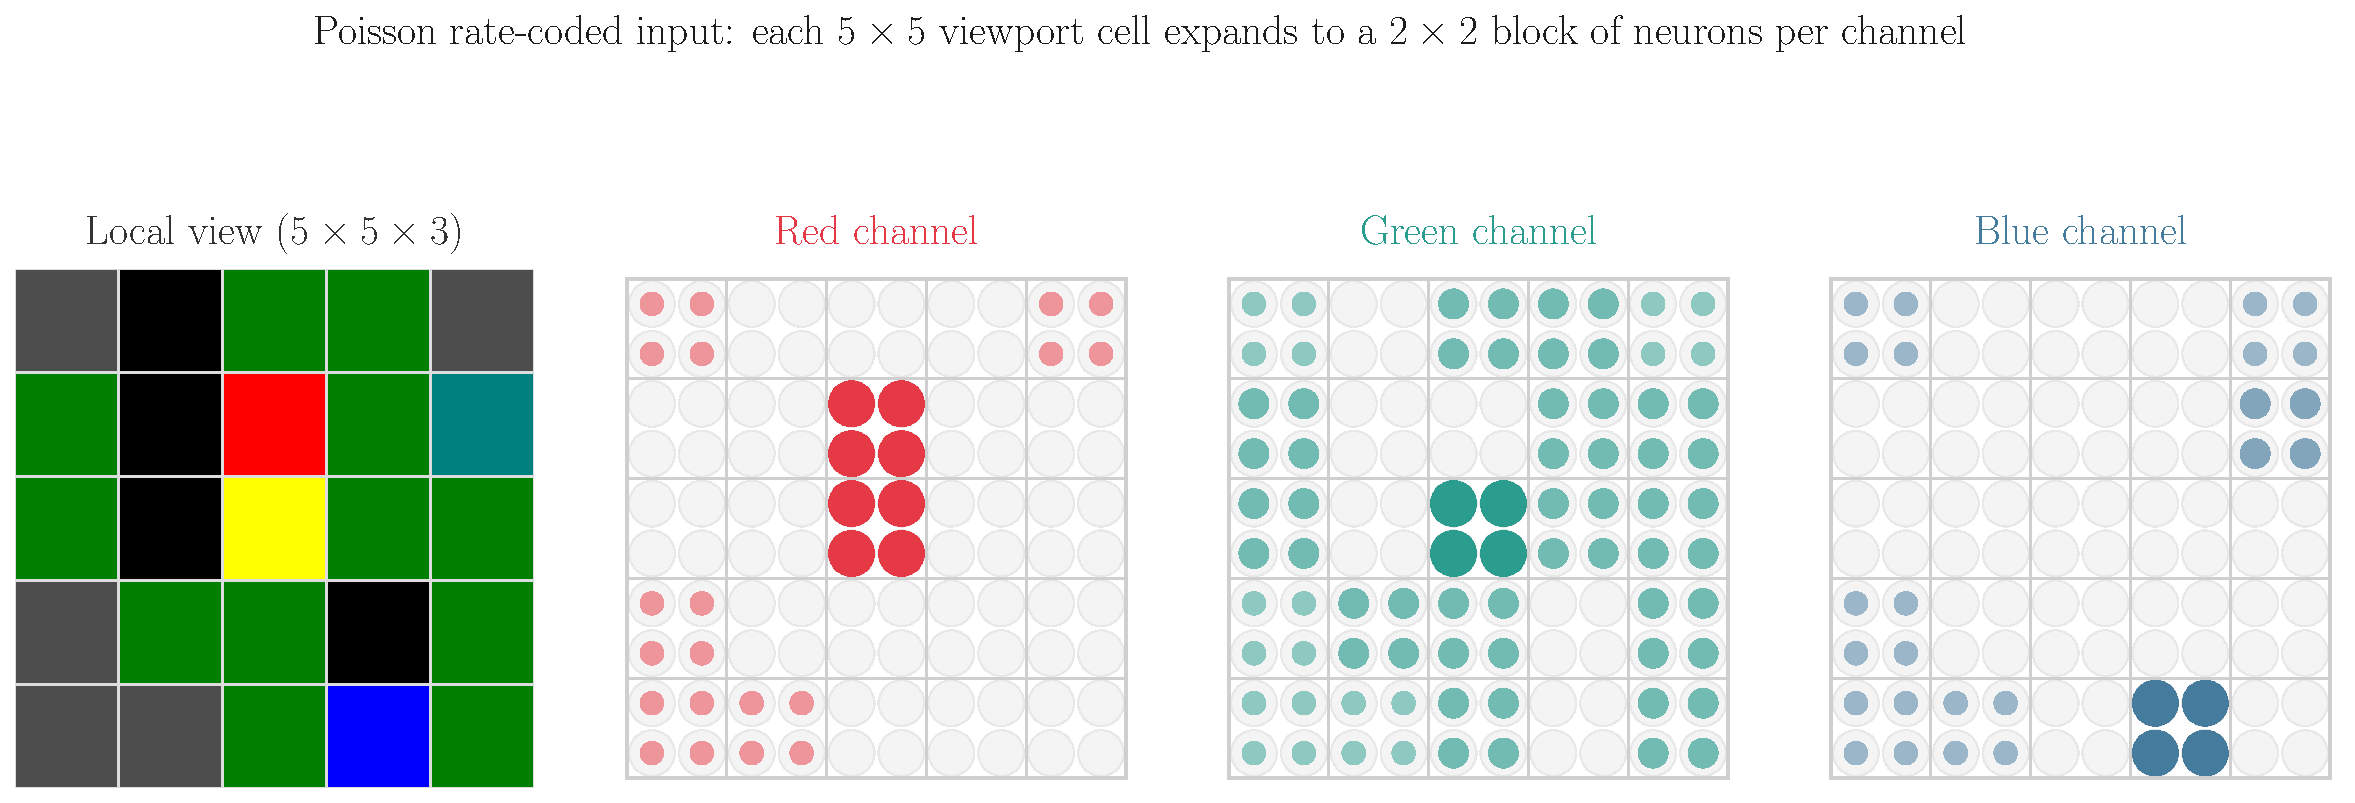
\includegraphics[width=1.0\textwidth]{images/poisson_input_encoding.pdf}
    \caption[Poisson rate-coded input encoding]{Poisson rate-coded encoding of the agent's observation. The $5\times5$ 
    view (left) is upscaled so that each cell becomes a $2\times2$ block of input neurons 
    in each of the three channels. Each neuron fires as a sequence of Bernoulli trials whose 
    probability is proportional to the corresponding channel intensity, up to a maximum of 
    $p_{max}$. Circle size and opacity are proportional to the firing probability.}
    \label{fig:poisson_input}
\end{figure}


\subsubsection{Agent's Input}
Before describing the individual tasks, we first introduce the common way in which 
all agents perceive their environment. Each agent observes a small grid-shaped view of the environment, encoded as a set of spike 
trains that the spiking network can process directly.

Concretely, the observation is a grid with three channels, which encode the different 
elements of the environment through distinct color intensities. This compact image is then upscaled 
so that each cell of the view is represented by a small $U \times U$ block of input neurons per 
channel, where $U$ is the upsampling scale, and every neuron is converted into a Poisson spike train whose firing probability is 
proportional to the corresponding channel intensity, up to a maximum of $p_{max}$. In this way, 
a brighter input drives its neuron to fire more often, while an empty cell remains silent, and 
the continuous observation is turned into the temporal, event-based signal that the network 
consumes at each step.

Figure~\ref{fig:poisson_input} illustrates this encoding for a representative observation. 
The left panel shows the view as the agent receives it, and the three panels on the right 
show the resulting per-channel grids of input neurons, where the size and opacity of each circle 
reflect how strongly that neuron fires. This same scheme is used across all the environments 
considered in this chapter; only the meaning of the elements in the scene changes from one task 
to another.

\subsubsection{Environment 1: Snake} 
\begin{figure}[H]
    \centering
    
\includegraphics[width=0.3\linewidth]{snake.png}
    \caption[The Snake environment]{The Snake environment, rendered as an RGB image: the green cells trace the
    snake's body, the red cell marks the food, and the grey border denotes the
    walls. The agent perceives only a $5\times5$ window centred on the head.}
    \label{fig:placeholder}
\end{figure}

The Snake environment places the agent in a grid world in which it must navigate a
growing body to collect food pellets without colliding with itself or the walls. The agent
receives a local pixel observation centred on the head, covering a fixed window of
$5 \times 5$ cells rendered as an RGB image.

This environment probes several distinct capabilities simultaneously. At the level of
reactive control, the agent must avoid immediate self-collision, which requires integrating
the current direction of motion with the local layout of the body. Crucially, reversing
direction is physically prevented, so the agent must commit to actions whose consequences
unfold over multiple steps and cannot be corrected immediately. This tests whether the
learning rule can shape a policy that avoids locally attractive but globally harmful actions,
and whether the eligibility traces retain sufficient signal to assign credit across the
relevant horizon.

The reward signal is relatively sparse, a positive reward is delivered only upon eating a pellet,
and a strong negative reward upon death, with no intermediate shaping. Whether the
algorithm can propagate this sparse signal back across the steps that preceded it is
therefore directly observable from the agent's ability to collect food consistently.

\subsubsection{Environment 2: Pac-Man}
\begin{figure}[H]
    \centering
    
\includegraphics[width=0.35\linewidth]{pac-man.png}
    \caption[The Pac-Man environment]{The Pac-Man environment. The agent (yellow) collects pellets and power
    capsules while avoiding ghosts; eating a capsule briefly frightens the ghosts (white),
    making them edible before they return to pursuing (orange). Walls restrict the legal
    moves differently at each position, and rewards span several magnitudes dependant on pellets,
    frightened-ghost captures, and the penalty for being caught.}
    \label{fig:placeholder}
\end{figure}
The Pac-Man environment places the agent in a maze populated by food pellets, power
capsules, and ghost enemies. The agent receives a local pixel observation centred on its
current position and must navigate the maze to collect food while avoiding or, when
powered up, pursuing ghosts.

Unlike the preceding environment, Pac-Man combines several sources of reward
structure simultaneously. Positive rewards arrive at irregular intervals as pellets are
collected, large positive rewards are available for eating frightened ghosts, and a strong
negative reward follows capture by an active ghost. The mix of timescales (dense local
rewards from pellet collection interleaved with rare but high-magnitude events from ghost
interactions) could allows us to evaluate whether the learning rule can simultaneously support
short-horizon reactive behavior and longer-horizon strategic planning within the same
task.

A distinctive feature of this environment is the prevalence of invalid actions. At any
given position, walls constrain the agent to a strict subset of the four cardinal directions,
and the legal set changes at every step as the agent moves through the maze. This
requires the policy to handle a persistent mismatch between the network's fixed
four-dimensional output and the variable-cardinality legal set, and provides a direct test
of how the algorithm manages probability mass assigned to unavailable actions. 

The ghost dynamics introduce a non-stationary element, ghost behavior switches between
chasing and retreating depending on the capsule state, and the agent must learn to
condition its behavior on this mode, which is only partially observable from the local
viewport. This tests the network's ability to use its recurrent state to disambiguate
situations that appear similar from a single-step observation, providing evidence about
the practical utility of the recurrent dynamics for contextual adaptation.

The environment is the classic implementation from the UC Berkeley
CS188 Pac-Man AI projects~\citep{denero2010pacman},\footnote{\url{https://ai.berkeley.edu}}
which we accessed through a Python~3.7 port provided by the thesis supervisor.
We extended this environment with procedurally generated layouts and a
continuing-task formulation without episodic resets.

\subsection{The Randomized Layouts Problem}

In this problem, the agent is placed in a $15 \times 15$ maze enclosed by walls and partially filled with interior obstacles that divide the space into a connected network of corridors. The maze is fully connected, so every open cell (and therefore every item and ghost) is reachable from any starting position. Scattered throughout the corridors are food pellets, two power pellets, and two ghosts, and the agent controls Pac-Man, whose objective is to clear the maze of food while avoiding the ghosts.

Crucially, the maze and the placement of all entities differ in every episode. The agent never sees the same configuration twice: walls, food, power pellets, ghosts, and its own starting position are all arranged differently each time. As a result, the agent cannot rely on a memorized map of the environment. It must instead learn a policy that operates entirely from its current local observation, generalizing across the wall configurations and entity placements it encounters.

At each step, the agent perceives a local window centered on Pac-Man and selects one of four movement directions. The reward reflects the outcome of each action, the agent receives a reward of $+1.0$ for eating a food pellet or a power pellet, $+2.0$ for catching a ghost that has been made vulnerable, and $-2.0$ when it is caught by an active ghost. Ordinary movement through empty corridors yields no reward, so the agent is neither rewarded nor penalized for exploration in itself, but exploration is rewarded anyway through the pellets. This scheme drives the agent to consume food and exploit vulnerable ghosts while avoiding fatal encounters.

The agent does not perceive the maze in its entirety, at each step it only observes a small $5 \times 5$ window centered on Pac-Man, leaving the rest of the maze hidden. It must therefore act under partial observability, inferring how to move toward food and away from ghosts from a narrow local view. This restricted window is a double-edged design choice. On the one hand, it limits the information available to the agent, hiding distant food and approaching ghosts and forcing it to act on incomplete knowledge. On the other hand, because the window is always centered on Pac-Man, the observation is inherently translation-invariant and low-dimensional meaning that the same local pattern always maps to the same relative situation regardless of where Pac-Man is in the maze. This compactness and consistency greatly reduce the size of the input space the network must learn to interpret, which accelerates learning and makes the policy easier to generalize across layouts.

The balance between partial observability and learning velocity is also shaped by the nature of the model itself. Because we employ SRNNs, partial observability is far less limiting than it would be for a purely feedforward architecture. The recurrent connectivity endows the network with an internal memory, information from previous observations persists in the network state and is integrated over time, allowing the agent to build an implicit, evolving representation of its surroundings as it moves. In effect, the network can compensate for the narrowness of any single observation by accumulating evidence across successive steps, so the $5 \times 5$ window restricts the instantaneous input far more than it restricts the information actually available to the policy.

Finally, although the constantly changing layout would in principle make this task harder than solving a single fixed maze, in the context we work in this variability is in fact necessary. The algorithms we employ are prone to action overcommitment, whereby an initial bias toward particular actions or strategies is quickly reinforced and ends up nullifying further learning. By continually varying the layout, we prevent such premature convergence and force the agent to keep learning a general, reactive strategy for collecting food and evading ghosts rather than a solution tailored to any single configuration. For this environment we used per-episode updates, as per-action updates were found to reliably collapse training.

\subsubsection{Environment 3: Connect Four}
\begin{figure}[H]
    \centering
    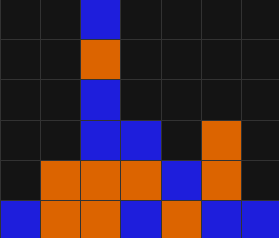
\includegraphics[width=0.35\linewidth]{connect-4.png}
    \caption[The Connect Four environment]{The Connect Four environment. Tokens are dropped into the columns of a
    $6\times7$ grid, with the agent's and opponent's pieces shown in blue and orange, and
    the goal is to align four in a row before the opponent. The full board is rendered as
    an RGB image at every turn, and rewards are sparse: $+1$ for a win, $-1$ for a loss,
    and $0$ otherwise.}
    \label{fig:placeholder}
\end{figure}
The Connect Four environment presents the agent with a two-player, turn-based board
game in which pieces are dropped into columns of a $6 \times 7$ grid and the objective
is to form a horizontal, vertical, or diagonal line of four consecutive pieces before the
opponent does. The full board state is rendered as a pixel image and provided to the
agent at each turn.

The reward structure is maximally sparse: a reward of $+1$ is delivered upon winning,
$-1$ upon losing, and $0$ at every intermediate step. The consequence of any individual
move may only become apparent several turns later when a winning or losing configuration
is completed. This makes the environment a direct test of long-horizon action credit
assignment, because the learning rule must attribute the terminal outcome back to the sequence
of placements that caused it, with no intermediate signal to guide this attribution.

The opponent is configured as a heuristic agent that blocks the agent's immediate winning
moves when it detects them, and wins in one-move if it detects the win, but does not plan beyond a single move ahead and can
therefore miss multi-step threats. The agent must learn to build attacking and defensive
patterns that exploit this limited lookahead, which requires recognizing recurring board
configurations and understanding which structural features carry strategic significance.
This makes pattern recognition over a structured spatial input a central demand of the
task, and allows us to evaluate whether the network's spatial organization supports the
development of such representations.

The combination of maximally sparse rewards, a reactive but imperfect opponent, and
spatially structured winning conditions makes Connect Four a clean testbed for isolating
the credit assignment and pattern recognition capabilities of the learning rule, with
outcomes that are directly interpretable in terms of win, loss, and draw rates.

Taken together, the three environments are complementary. Snake provides a controlled setting for studying sparse credit assignment,
reactive commitment, and scalable working memory, Pac-Man introduces a richer and more mixed setting in which dense
and sparse rewards coexist, illegal actions are pervasive, and the relevant context is
partially observable, allowing us to evaluate the algorithm's behavior when multiple
demands are present simultaneously and Connect Four isolates long-horizon
credit assignment and spatial pattern recognition under maximally sparse rewards and a
structured opponent. For this environment we used per-episode updates, as per-action updates were found to reliably collapse training.